\documentclass[11pt]{article}
\usepackage[margin=0.5in]{geometry}
\usepackage{todonotes}
\usepackage{graphicx}
\usepackage{listings}
\usepackage{color}
\usepackage{hyperref}
\usepackage{multirow}
\usepackage{pifont}
\usepackage{xcolor,colortbl}
\usepackage{hyperref}
\hypersetup{colorlinks=true,linkcolor=blue!50!black,citecolor=blue!75!black,filecolor=black,urlcolor=blue!75!black}
\usepackage{amsmath}
\usepackage{amssymb}
\usepackage{xspace}
\usepackage{makecell}
\usepackage{ulem} % provides sout
\usepackage[frozencache=true,cachedir=minted-cache]{minted} 
\usepackage[htt]{hyphenat}      
\usepackage{subcaption}
\usepackage{graphicx,import}
\usepackage{booktabs}


% \usepackage{subfigure}

\newcommand{\tristan}[1]{\color{orange}\textbf{From Tristan:} #1\color{black}\xspace}
\newcommand{\tristanmod}[2]{\color{orange}\sout{#1} #2\color{black}\xspace}
\newcommand{\gkmod}[2]{\color{purple}\sout{#1} #2\color{black}\xspace}

\newcommand{\Yohan}[1]{\color{green!75!black}\textbf{Yohan:} #1\color{black}\xspace}
\newcommand{\cross}[0]{\cellcolor{red!65}\ding{53}}
\newcommand{\valid}[0]{\cellcolor{green!75!black}\ding{51}}
\newcommand{\warn}[0]{\cellcolor{orange!75}?}
\newcommand{\na}[0]{\cellcolor{gray!25}}
\newcommand{\s}[1]{\cellcolor{cyan!25}#1}
\newcommand{\scross}[0]{\ding{53}~}
\newcommand{\svalid}[0]{\ding{51}~}
\newcommand{\swarn}[0]{?~}
\newcommand{\pytracer}[0]{PyTracer\xspace}

\setlength{\arrayrulewidth}{0.1pt}


\newcommand{\discreteCosineRF}{ \href{https://docs.scipy.org/doc/scipy/tutorial/fft.html\#discrete-cosine-transforms}{discrete\_cosine\_transform} }
\newcommand{\fftOneDRf}{
\href{https://docs.scipy.org/doc/scipy/tutorial/fft.html\#d-discrete-fourier-transforms}{fft\_1D}
}
    
\newcommand{\fftTwoDRf}{
\href{https://docs.scipy.org/doc/scipy/tutorial/fft.html\#and-n-d-discrete-fourier-transforms}{fft\_2D}
}

\newcommand{\interOneDRf}{
\href{https://docs.scipy.org/doc/scipy/tutorial/interpolate.html\#d-interpolation-interp1d}{interpolation\_1D} 
}

\newcommand{\multiRf}{
\href{https://docs.scipy.org/doc/scipy/tutorial/interpolate.html\#multivariate-data-interpolation-griddata}{multivariate\_data} 
}

\newcommand{\bsplineRf}{
\href{https://docs.scipy.org/doc/scipy/tutorial/signal.html\#b-splines}{bspline}  
}

\newcommand{\splineOneDRf}{
    \href{https://docs.scipy.org/doc/scipy/tutorial/interpolate.html\#spline-interpolation-in-1-d-procedural-interpolate-splxxx}{
    spline\_1D} 
}

\newcommand{\splineTwoDRf}{
    \href{https://docs.scipy.org/doc/scipy/tutorial/interpolate.html\#d-spline-representation-procedural-bisplrep}{
    spline\_2D} 
}

\newcommand{\bfgsRf}{
    \href{https://docs.scipy.org/doc/scipy/tutorial/optimize.html\#broyden-fletcher-goldfarb-shanno-algorithm-method-bfgs}{broyden\_fletcher\_goldfarb\_shanno} 
}

\newcommand{\globalRf}{
    \href{https://docs.scipy.org/doc/scipy/tutorial/optimize.html\#global-optimization}{
    global\_optimization} 
}

\newcommand{\slsqpRf}{
    \href{https://docs.scipy.org/doc/scipy/tutorial/optimize.html\#sequential-least-squares-programming-slsqp-algorithm-method-slsqp}{
    slsqp} 
}
    
\newcommand{\lsmRf}{
    \href{https://docs.scipy.org/doc/scipy/tutorial/optimize.html\#least-squares-minimization-least-squares}{
    least\_square\_minimization} 
}

\newcommand{\nelderRf}{
    \href{https://docs.scipy.org/doc/scipy/tutorial/optimize.html\#nelder-mead-simplex-algorithm-method-nelder-mead}{nelder\_mead\_simplex}
}

\newcommand{\ncgRf}{
    \href{https://docs.scipy.org/doc/scipy/tutorial/optimize.html\#newton-conjugate-gradient-algorithm-method-newton-cg}{
    newton\_conjugate\_gradient}  
}

\newcommand{\rootRf}{
    \href{https://docs.scipy.org/doc/scipy/tutorial/optimize.html\#sets-of-equations}{
    root\_findings}  
}

\newcommand{\rootLargRf}{
    \href{https://docs.scipy.org/doc/scipy/tutorial/optimize.html\#root-finding-for-large-problems}{
    root\_finding\_large} 
}

\newcommand{\rootLargePredRf}{
    \href{https://docs.scipy.org/doc/scipy/tutorial/optimize.html\#still-too-slow-preconditioning}{
    root\_finding\_large\_preconditioned} 
}

\newcommand{\trustExactRf}{
    \href{https://docs.scipy.org/doc/scipy/tutorial/optimize.html\#trust-region-nearly-exact-algorithm-method-trust-exact}{
    trust\_region\_exact} 
}

\newcommand{\trustTruncRf}{
    \href{https://docs.scipy.org/doc/scipy/tutorial/optimize.html\#trust-region-truncated-generalized-lanczos-conjugate-gradient-algorithm-method-trust-krylov}{
    trust\_region\_truncated\_generalized\_lanczos} 
}

\newcommand{\trustNCGRf}{
    \href{https://docs.scipy.org/doc/scipy/tutorial/optimize.html\#trust-region-newton-conjugate-gradient-algorithm-method-trust-ncg}{
    trust\_region\_newton\_conjugate\_gradient} 
}

\newcommand{\AdaboostRf}{
    \href{https://scikit-learn.org/stable/auto_examples/ensemble/plot_adaboost_regression.html}{AdaBoost} 
}

\newcommand{\brrRf}{
    \href{https://scikit-learn.org/stable/auto_examples/linear_model/plot_bayesian_ridge.html}{Bayesian Ridge Regression} 
}

\newcommand{\onlineClassifierComparisonRf}{
    \href{https://scikit-learn.org/stable/auto_examples/linear_model/plot_sgd_comparison.html}{Online classifier comparison} 
}

\newcommand{\kmeansRf}{
    \href{https://scikit-learn.org/stable/auto_examples/cluster/plot_cluster_iris.html}{K-Means Clustering}  
}

\newcommand{\covarianceRf}{
    \href{https://scikit-learn.org/stable/auto_examples/covariance/plot_mahalanobis_distances.html}{Covariance estimation}  
}

\newcommand{\decisionRf}{
    \href{https://scikit-learn.org/stable/auto_examples/tree/plot_tree_regression.html}{Decision Tree Regression}
}

\newcommand{\digitsRf}{
    \href{https://scikit-learn.org/stable/auto_examples/linear_model/plot_sgd_comparison.html}{Digits Classification} 
}

\newcommand{\faceRf}{
    \href{https://scikit-learn.org/stable/auto_examples/decomposition/plot_faces_decomposition.html}{Face Recognition} 
}

\newcommand{\penaltyRf}{
    \href{https://scikit-learn.org/stable/auto_examples/linear_model/plot_logistic_l1_l2_sparsity.html}{L1 Penalty} 
}

\newcommand{\lassoRf}{
    \href{https://scikit-learn.org/stable/auto_examples/linear_model/plot_lasso_and_elasticnet.html}{Lasso and Elastic Net} 
}

\newcommand{\hyperplaneRf}{
    \href{https://scikit-learn.org/stable/auto_examples/linear_model/plot_sgd_separating_hyperplane.html}{Separating hyperplane} 
}

\newcommand{\mnistRf}{
    \href{https://scikit-learn.org/stable/auto_examples/linear_model/plot_sparse_logistic_regression_mnist.html}{MNIST classification} 
}

\newcommand{\multitaskRf}{
    \href{https://scikit-learn.org/stable/auto_examples/linear_model/plot_multi_task_lasso_support.html}{Multitask Lasso}  
}

\newcommand{\ompRf}{
    \href{https://scikit-learn.org/stable/auto_examples/linear_model/plot_omp.html}{Orthogonal Matching} 
}

\newcommand{\pcaRf}{
    \href{https://scikit-learn.org/stable/auto_examples/decomposition/plot_pca_iris.html}{PCA decomposition}  
}

\newcommand{\robustRf}{
    \href{https://scikit-learn.org/stable/auto_examples/linear_model/plot_ransac.html}{Robust Linear Regression} 
}

\newcommand{\toyRf}{
    \href{https://scikit-learn.org/stable/auto_examples/cluster/plot_segmentation_toy.html\#sphx-glr-auto-examples-cluster-plot-segmentation-toy-py}{Segmentation toy}  
}

\newcommand{\svmRf}{
    \href{https://scikit-learn.org/stable/auto_examples/svm/plot_separating_hyperplane_unbalanced.html\#sphx-glr-auto-examples-svm-plot-separating-hyperplane-unbalanced-py}{SVM}  
}

\newcommand{\tomographyRf}{
    \href{https://scikit-learn.org/stable/auto_examples/applications/plot_tomography_l1_reconstruction.html\#sphx-glr-auto-examples-applications-plot-tomography-l1-reconstruction-py}{
    Tomography} 
}

\newcommand{\weightedRf}{
    \href{https://scikit-learn.org/stable/auto_examples/linear_model/plot_sgd_weighted_samples.html\#sphx-glr-auto-examples-linear-model-plot-sgd-weighted-samples-py}{SGD weighted samples} 
}


\usepackage{tabularx} % provides tabularx to adjust table column sizes to page size
% define thickline for use in tables
\makeatletter
\newcommand{\thickhline}{%
    \noalign {\ifnum 0=`}\fi \hrule height 1pt
    \futurelet \reserved@a \@xhline
}
\newcolumntype{"}{@{\hskip\tabcolsep\vrule width 1pt\hskip\tabcolsep}}
\makeatother


\lstdefinestyle{customPython}{
  belowcaptionskip=1\baselineskip,
  breaklines=true,
  xleftmargin=\parindent,
  language=Python,
  showstringspaces=false,
  basicstyle=\scriptsize\ttfamily,
  keywordstyle=\bfseries\color[rgb]{0.580, 0.000, 0.827},
  %{purple!40!lightgray},
  commentstyle=\itshape\color{green!40!black},
  identifierstyle=\bfseries\color{cyan!75!black},
  stringstyle=\color{orange},
  deletekeywords={double,float},
  classoffset=1, % starting new class
  otherkeywords={double,float},
  morekeywords={double,float},
  keywordstyle=\bfseries\color{green!55!black},
  classoffset=0
}

\lstdefinestyle{customC}{
  belowcaptionskip=1\baselineskip,
  breaklines=true,
  xleftmargin=\parindent,
  language=C,
  showstringspaces=false,
  basicstyle=\scriptsize\ttfamily,
  keywordstyle=\bfseries\color[rgb]{0.580, 0.000, 0.827},
  %{purple!40!lightgray},
  commentstyle=\itshape\color{green!40!black},
  identifierstyle=\bfseries\color{cyan!75!black},
  stringstyle=\color{orange},
  deletekeywords={double,float},
  classoffset=1, % starting new class
  otherkeywords={double,float},
  morekeywords={double,float},
  keywordstyle=\bfseries\color{green!55!black},
  classoffset=0
}


\begin{document}

\makeatletter
\let\orig@lstnumber=\thelstnumber
\newcommand\lstsetnumber[1]{\gdef\thelstnumber{#1}}
\newcommand\lstresetnumber{\global\let\thelstnumber=\orig@lstnumber}
\makeatother

\title{PyTracer: Automatically profiling numerical instabilities in Python}
\author{Yohan Chatelain$^1$, Nigel Yong$^1$,  Gregory Kiar$^2$,  Tristan Glatard$^1$\\
$^1$Department of Computer Science and Software Engineering, Concordia University, Montreal, Canada\\
$^2$Center for the Developing Brain, Child Mind Institute, New York, NY, USA}
\date{\textit{This work has been submitted to the IEEE for possible publication. 
Copyright may be transferred without notice, after which this version may no 
longer be accessible.}}
\maketitle


\begin{abstract}
Numerical stability is a crucial requirement of reliable scientific computing. However, despite the pervasiveness of Python in data science, analyzing large Python programs remains challenging due to the lack of scalable numerical analysis tools available for this language. To fill this gap, we developed \pytracer, a profiler to quantify numerical instability in Python applications. \pytracer transparently instruments Python code to produce numerical traces and visualize them interactively in a Plotly dashboard. We designed \pytracer to be agnostic to numerical noise model , allowing for tool evaluation through Monte-Carlo Arithmetic, random rounding, random data perturbation, or structured noise for a particular application. We illustrate \pytracer's capabilities by testing the numerical stability of key functions in both SciPy and Scikit-learn, two dominant Python libraries for mathematical modeling. Through these evaluations, we demonstrate \pytracer as a scalable, automatic, and generic framework for numerical profiling in Python.
% Numerical stability is a crucial requirement of reliable scientific computing. However, despite the pervasiveness of Python in data science, analyzing large Python programs remains challenging due to the lack of scalable numerical analysis tools available for this language. To address this issue, we developed \pytracer, a profiler to quantify numerical instability in Python applications. \pytracer automatically instruments Python code to produce numerical traces and visualize them interactively in a Plotly dashboard.
% \pytracer is designed to work with any type of numerical noise model, including Monte-Carlo Arithmetic, random rounding or random data perturbations. We illustrate \pytracer's capabilities by testing the numerical stability of key functions in the SciPy and Scikit-learn Python libraries. Finally, \pytracer slows down executions by only $3.5 \times$ on average.
% \tristan{Add one sentence to summarize the findings} 
\end{abstract}

\section{Introduction}

The scientific Python ecosystem has become a central component of data
analyses in recent years, owing to its rich offering of data manipulation, array programming,
numerical analysis, and visualization tools. In particular, libraries such
as NumPy~\cite{harris2020array}, SciPy~\cite{virtanen2020scipy}, scikit-learn~\cite{pedregosa2011scikit} or PyTorch~\cite{paszke2019pytorch} are used in hundreds of publications each year, and serve as a reference set of high-quality open-source core scientific libraries. Researchers have built numerous domain-specific software tools from this ecosystem, leveraging Python's simplicity and flexibility. 

Numerical stability is a crucial requirement of reliable scientific data
processing. In unstable analyses, small numerical perturbations introduced by data noise, software and hardware updates, or parallelization have potential to introduce substantial deviations in final results, leading to potentially different scientific conclusions, ultimately threatening the reliability of computational analyses. To prevent this, numerical stability analyses need to be conducted systematically, however, no practical tool currently exists to conduct such analyses for Python programs.

We present PyTracer, a numerical stability profiling and visualization tool for Python programs.
\pytracer adopts a dynamic approach that evaluates numerical stability using program execution traces, and is applicable to large programs without manual intervention. The transparent nature of \pytracer is particularly valuable in contrast to theoretical approaches based on condition numbers or backward error analysis, which require detailed modeling of the program and its numerical implementation. Similarly, static code analysis techniques hardly scale to large code bases, particularly in dynamically-typed languages such as Python.

\pytracer estimates the variability of floating-point variables by combining program traces obtained with different numerical perturbations, which requires (1) generating numerically-perturbed executions, (2) tracing floating-point computations along program executions, and (3) visualizing stability evaluations. \pytracer addresses these requirements with (1) a ``fuzzy" Python interpreter instrumented with Monte-Carlo arithmetic, (2) a dynamic instrumentation of Python functions, modules, and classes through meta-programming, (3) an interactive Plotly dashboard to visualize stability measures throughout program executions.

This manuscript presents the design of \pytracer and demonstrates its potential in various use cases. 
Through stability evaluations of the
SciPy and scikit-learn libraries, we demonstrate \pytracer as a practical solution to review the numerical stability of extensive code bases. 
%All information was obtained through \pytracer, visualized separately for improved customizability.
%\tristan{this is a weird place to mention this ^^}



\section{\pytracer design}

% \subsection{Pytracer workflow}
\pytracer adopts the three-step workflow shown in Figure~\ref{fig:workflow}. First, \pytracer uses \textit{monkey patching} to replace the functions called by the application with a wrapper that saves their arguments and returned values in a trace file.
% \gkmod{}{Q: This is conceptually similar to a decorator, no? If so, perhaps it is worth mentioning} \Yohan{Conceptually, monkey patching is the ability to dynamically change a class or a module. So it's more powerful than the decorators. But yes we use monkey-patching to automatically decorate the functions.}
Second, it executes the application multiple times with noise injection, and aggregates the resulting trace files to compute summary statistics about each traced variable. Finally, a Plotly dashboard provides interactive visualizations highlighting unstable code sections.

% \tristan{mention monkey patching}

\begin{figure}
    \centering
    \includegraphics[width=\linewidth]{figure/workflow.pdf}
    \caption{Pytracer workflow
    % \gkmod{}{Note: replace "Execution" with "Multiple Independent Executions", and maybe move it to be between the gears and the pkl files.}
    }
    \label{fig:workflow}
\end{figure}

\subsection{Python code instrumentation}

%\tristan{``Instrumentation" should appear in Figure 1}


\pytracer dynamically instruments Python modules
without requiring source code modifications in the application.
To do so, it creates a new, instrumented version of each module that preserves its original attributes so that the application can transparently use it.
% \gkmod{}{Note: this form of monkey patching is basically global and transparent decorating, right?} \Yohan{Yes}
By default, \pytracer instruments all the attributes
in a given module except the special ones of the form \texttt{\_\_*\_\_}, which is common for reserved Python methods.
However, some attributes are not writable. In this case, \pytracer preservers the original attributes and warns the user. The user can also restrict the list of traced attributes through
an inclusion/exclusion mechanism. The main advantage of this instrumentation approach is the lack of required modification in the application source code, in contrast with decorator-based approaches. In addition, this technique is scalable and applicable in read-only environments such as Singularity containers or HPC clusters.





\subsubsection{Intercepting module import}

Python loads modules through an import mechanism triggered by the \texttt{import} keyword that involves two objects: \texttt{finders} and \texttt{loaders}. \texttt{Finders} search for packages (or 
namespaces\footnote{Python distinguishes between \texttt{regular} and \texttt{namespace} packages.
A regular package is a directory that contains a \_\_init\_\_.py file and potentially subdirectories (sub-packages) 
that contain themselves a \texttt{\_\_init\_\_.py} file and so on recursively. 
The package hierarchy follows those of the directory. 
Namespace packages introduced in Python 3.3 (\href{https://www.python.org/dev/peps/pep-0420/}{PEP 420}) do not contain an
\_\_init\_\_.py file and allow for flexible directory structures. Hence, parts of the package can be located in zip files, on the network, or in separated directories. There are no functional differences between both types of packages.}) on the local storage --- such as standard packages installed through the pip package manager --- or on a distant server.
\texttt{Finders} do not load modules. Instead, they return a specification (\texttt{spec} object) that includes 
information on where to find and how to load modules.
\texttt{Loaders} create module objects, initialize them, and fill import-related attributes 
such as \texttt{\_\_spec\_\_}. 
\texttt{Loaders} then execute modules and populate their namespace. Finally, modules are bound to their import name in the \texttt{sys.modules} dictionary.


Python supports custom \texttt{finder} classes registered in the \texttt{sys.meta\_path} list.
When Python encounters an \texttt{import} statement, it first looks for an existing binding in \texttt{sys.modules} and then iterates over the \texttt{finder} classes in the \texttt{sys.meta\_path} list until it finds the module. \pytracer adds a custom \texttt{finder} class at the head of \texttt{sys.meta\_path} that intercepts
the module import and creates the module with a custom \texttt{loader} class.

\pytracer's \texttt{loader} class first loads the original module, then copies it as a new instance of the \texttt{ModuleType} class. It then calls the appropriate instrumentation function for each attribute depending on its type (function, class, or instances) and replaces the original module in the \texttt{sys.modules} map with the instrumented version. Finally, it updates all existing references to the original module contained in the global symbol table.
As a result, the application will transparently call the instrumented module.

% \tristan{is the non-instrumented version ever added to sys.modules? If so, could this lead to race conditions? If not, replace with ``adds the instrumented module to the sys.modules map"}. 
% \Yohan{Yes, it replaces the original module. You can't have a race-condition since sys.modules is a dict with only one value for a given key. The trick is that the wrapped module keeps a reference to the original module, it's just that this reference is invisible for the others object since it's not in sys.modules and globals. By the way, Pytracer needs to update all possible references that original objects may hold, like functions in \_\_dict\_\_ attributes or locals references in \_\_globals\_\_ for example.}

% \pytracer intercepts the modules loaded with the \texttt{Finder} and \texttt{Loader} mechanisms \tristan{is it restrictive? Are there other mechanisms?}.
% The Finder searches the loader of a module that is being imported while the 
% Loader loads and initializes the module. \pytracer adds \tristan{overrides?} a new Finder and Loader on top of the default ones
% to intercept imports and to instrument modules selected by the user. This mechanism allows returning 
% the original module in the instrumentation code and returning the instrumented module in the targeted application
% without modifying its actual code.

\subsubsection{Instrumenting module functions}

Listings~\ref{fig:wrapper_creation} and~\ref{fig:generic_wrapper} show \pytracer's function instrumentation mechanism.
For each function to instrument, \pytracer's \texttt{loader} class creates a wrapper function, dynamically compiles it with the \texttt{compile} builtin function, and substitutes it for the original module function.  Although simple, this technique does not apply to callable class instances, i.e., class instances that have a \texttt{\_\_call\_\_} attribute and are not of type \texttt{FunctionType}. Indeed, applying the wrapper technique would 1) modify the type of the class instance to \texttt{FunctionType}, which could cause syntax and semantic errors, and 2) mask class attributes, leading to \texttt{AttributeError} exceptions.
\pytracer overrides the \texttt{\_\_call\_\_} attribute with the wrapper function when possible to overcome this issue.
When the \texttt{\_\_call\_\_} attribute is not writable,  Pytracer does not instrument the class and returns a warning. 

% \tristan{add docstrings to all Python code examples and clarify captions accordingly: you don't need to explain the meaning of each attribute in the caption if it's in the docstring. The caption can focus on the main functionality, reusing the text currently in 3.1.5.}
% \Yohan{TODO}

% Listing~\ref{fig:wrapper_creation} shows how functions are instrumented.
% This function takes as inputs the information about the function to instrument (module name and full qualified name),
% the function itself, and the actual name of the function. It then creates a wrapper around the actual wrapper
% (\texttt{generic\_wrapper}) that will save the values in trace files. Instead of passing the function, we pass the function's identifier, which is a unique 64-bits integer that references each Python object. This identifier is available
% with the \texttt{id} builtin function. it allows to get rid of aliases and to avoid instrumenting functions twice.  \tristan{Summarize this paragraph in the figure caption}

% Listing~\ref{fig:generic_wrapper} shows what the instrumented code does. 
% It first unpacks the function's information to get the function's identifier to retrieve the original function.
% Then arguments are bound by creating a mapping from positional and keyword arguments to parameters, avoiding conflicts and mispositioning. It also allows getting names of arguments for the visualization.
% Once bound, the \texttt{inputs} function dumps the arguments in the pickle file.
% Finally, Pytracer calls the function with the correct arguments, dumps the result, and returns it. \tristan{Summarize this paragraph in the figure caption}

%
% we can employ a case by case strategy depending on the class (i.e. numpy ufunc) or simply ignore
% the instrumentation and let the original one.
% \tristan{add a sentence to explain how callable instances are instrumented}




\begin{listing}
    \centering
\begin{lstlisting}[language=Python,style=customPython]
def get_wrapper_function(module, qualname, name, function):
    """Returns the instrumented function as a string.
    This string will be compiled with the compile builtin function
    
    Parameters:
        module: Name of the function module
        qualname: Qualified name of the function
        name: Name of the function
        function: Python object function
        
    Returns:
        wrapper_code: The code source of the wrapper
    """
    function_id = id(function)
    info = (function_id, function_module, function_qualified_name)
    wrapper_code = f"""
    def {function_wrapper_name}(*args, **kwargs):
        return generic_wrapper({info},*args,**kwargs)"""
    return wrapper_code
\end{lstlisting}
    \caption{Function to create the instrumented version of a function.
    \pytracer uses the identifier of the function instead of the 
    actual function to handle aliases and avoid duplicate instrumentation.}
    \label{fig:wrapper_creation}
\end{listing}


\begin{listing}
    \centering
\begin{lstlisting}[language=Python,style=customPython,]
def generic_wrapper(self, info, *args, **kwargs):
    """Generic wrapper saving inputs and outputs of the wrapped function.
    The id_dict dict keeps a mapping between the original function identifier
    and itself. Arguments are binded to avoid mispositioning.
    Returns the actual output of the wrapped function.
    
    Parameters:
        info: Tuple with the function's id, function's module and function's name
        *args: Positional calling arguments
        **kwargs: Keyword calling arguments
    
    Returns:
        outputs: Outputs of the wrapped function
    """
    fid, fmodule, fname = info
    function = original_function_cache.id_dict[fid]
    bind = Binding(function, *args, **kwargs)
    stack = self.backtrace()
    time = elements()
    self.inputs(time=time,
                module_name=fmodule,
                function_name=fname,
                function=function,
                args=bind.arguments,
                backtrace=stack)
    outputs = function(*bind.args, **bind.kwargs)
    self.outputs(time=time,
                 module_name=fmodule,
                 function_name=fname,
                 function=function,
                 args=outputs,
                 backtrace=stack)
    return outputs
\end{lstlisting}
    \caption{\pytracer's generic wrapper function that saves
    the inputs and outputs of the wrapped function.}
    \label{fig:generic_wrapper}
\end{listing}


\subsubsection{Instrumenting classes}

\pytracer instruments classes by wrapping their callable attributes as described previously. 
This instrumentation preserves class types, which avoids type mismatches in the instrumented application.
However, classes that describe particular base types and NumPy's universal functions (class \texttt{ufunc}) contain read-only attributes that cannot be instrumented.
By default, \pytracer returns a warning when it encounters such classes. 

\subsubsection{Instrumenting class instances}

\pytracer automatically instruments class instances since it instruments classes. However, it cannot instrument or instantiate classes that have read-only attributes --- in particular class \texttt{ufunc}, --- which is problematic given their pervasiveness in scientific computing. In particular, NumPy's universal functions include
vectorized elementary mathematical and other prevalent functions. 
%\gkmod{ones}{Q: prevalent whats?}.
Universal functions are implemented in C, which prevents their modification.

To overcome this issue, \pytracer wraps the class instance into a transparent wrap class (\texttt{twc}) that overloads
1) function \texttt{\_\_getattribute\_\_}, called when an instance attribute is accessed --- instrumented to return the attributes from the original class, and 2) function \texttt{\_\_call\_\_}, used when an instance behaves like a function through the () operator --- instrumented with function \texttt{generic\_wrapper}.
% \gkmod{}{Note: the previous sentence is a bit hard to follow; the word "called" is used a lot so I got a bit lost.}
The \texttt{twc} returns the queried attribute of the instance instead of returning its attributes, allowing transparent access to the instance.  Finally, \pytracer overloads the builtin \texttt{type} function to preserve the type of the wrapped instance.

\subsubsection{Instrumenting iterators}

In functional programming, iterators traverse containers lazily, meaning that the next element in the sequence is only computed when the application uses it. This technique allows for the manipulation of virtually infinite sequences with finite memory. However, it implies that no complete mapping of the container returned by an iterator exists in memory since the application computes each element on the fly. Therefore, iterators are not serializable which implies that \pytracer cannot save them to output traces. 
A workaround would be to convert iterators into explicit containers, however, this would increase the memory footprint significantly. \pytracer, therefore, does not instrument non-builtin iterators.

% \begin{listing}
% \begin{minipage}[t]{0.4\linewidth}
%     \begin{lstlisting}[language=Python,style=customPython]
% >>> import numpy as np
% >>> x = np.array(range(10))
% >>> index = np.array([1,-1],dtype=int)
% >>> x[index]
% >>> array([1, 9])
%     \end{lstlisting}
% \end{minipage}
% \begin{minipage}[t]{0.4\linewidth}
%     \begin{lstlisting}[language=Python,style=customPython]
% >>> import numpy as np
% >>> x = np.array(range(10))
% >>> index = np.array([1,-1], dtype=object)
% >>> x[index]
% Traceback (most recent call last):
%   File "<stdin>", line 1, in <module>
% IndexError: arrays used as indices must be of integer (or boolean) type
%     \end{lstlisting}
% \end{minipage}
% \caption{Illustration of the issue of using \texttt{frompyfunc} function to convert function to \texttt{ufunc}. Left: original code. Right: instrumented code. 
% \tristan{This needs more explanation: where is the ufunc, what is the type returned by the original ufunc, and why does it crash in the instrumented version.} \Yohan{TODO}}
%     \label{fig:numpy_array_index_issue}
% \end{listing}

\subsection{Detecting numerical instabilities}

\pytracer detects numerical instabilities by computing summary statistics across multiple executions perturbed with numerical noise. While \pytracer's instrumentation, trace aggregation, and visualization work with various types of numerical noise, we experimented primarily with Monte-Carlo Arithmetic (MCA) as it is an accurate model for floating-point errors.

\subsubsection{Noise injection}
\label{sec:fuzzy}

Three  main  approaches  exist  to  detect  numerical  instabilities:  stochastic  arithmetic,  uncertainty  or  sensitivity analysis [23], and random seed analysis [11].  PyTracer is agnostic to the noise model used and therefore works for all methods mentioned.  For our use cases, we focus on stochastic arithmetic since it does not make any assumption about the noise model, in contrast to sensitivity analysis

Stochastic arithmetic leverages randomness to estimate numerical instabilities coming from the use of floating-point representations. The main idea is to treat round-off errors as random variables and characterize them statistically.
Monte Carlo Arithmetic (MCA)~\cite{parker1997monte} uses this principle by introducing two improvements:
(i) a virtual precision parameter, allowing to simulate reduced working precision, and (ii) different perturbation modes to introduce perturbations
on function inputs or output.
MCA replaces each floating-point number $x$ with a stochastic counterpart computed as:
\[
inexact(x) =  x + \beta^{e_x - t}\xi
\]
where $\beta$ is the number base, $e_x$ is the magnitude of $x$, $t$ the virtual precision and $\xi \in (-\frac{1}{2},\frac{1}{2})$ is a random uniform variable.
Virtual precision allows for the simulation of reduced working precision.
MCA can be applied in three modes: Random Rounding (RR), Precision Bounding (PB), and full MCA, which apply function $inexact$ to the output, the inputs, or both, respectively. While the RR mode is equivalent to stochastic rounding, the PB mode can also identify catastrophic cancellations.

Stochastic arithmetic quantifies numerical error using the number of significant digits $s$ estimated among the sampled values. A common formula to determine this number from MCA samples is presented in~\cite{parker1997monte}:
\begin{equation}
s = -\log_{\beta}{ \left| \dfrac{\sigma}{\mu} \right|} \label{eq:sig-digits}
\end{equation}
where $\mu$ and $\sigma$ are the sample mean and standard deviation of a variable sampled with MCA.  
Sohier et al.~\cite{sohier2018confidence} recently provided a generalization of this formula to include confidence intervals.

We enable MCA in Python programs via Verificarlo~\cite{verificarlo}, a clang-based compiler~\cite{lattner2008llvm} that replaces floating-point operations by a generic call to a configurable floating-point model. Several floating-point models are available~\cite{chatelain2019automatic,chatelain2019outils}, also called backends.
\pytracer leverages ``fuzzy"~\cite{kiar2020comparing}, a collection of software tools compiled with Verificarlo. In particular, fuzzy provides MCA-instrumented versions of the Python interpreter as well as the BLAS, LAPACK, NumPy, SciPy, and scikit-learn libraries, which enables MCA for a wide range of existing scientific Python programs. Fuzzy is available in Verificarlo's GitHub organization at \href{https://github.com/verificarlo/fuzzy}{\url{github.com/verificarlo/fuzzy}}.

% As the time of writing this article, fuzzy provides 5 levels of instrumentation (each level N including the lower levels):
% \begin{enumerate}
%     \item BLAS + LAPACK
%     \item Python interpreter
%     \item Numpy
%     \item SciPy
%     \item Scikit-learn
% \end{enumerate}

\subsubsection{Trace format}

\pytracer stores traces in the pickle format, a binary format to serialize Python objects.
The main advantages of the pickle format compared to other serialization approaches such as marshal or JSON are its ability to serialize most Python objects and its native compression.  In addition, pickle writes Python objects sequentially, which preserves the temporal ordering required by subsequent trace analyses.

Traces store numerical values at the granularity of function calls. When the application invokes a function, \pytracer saves a call input object containing contextual information (function's name, module's function, stacktrace) and the values of the function arguments. When the function returns, \pytracer saves a similar call output object containing the returned value. 


\subsubsection{Trace aggregation}

Once traces are available, \pytracer sequentially parses them and computes the mean, standard deviation, and the number of significant digits (as in Equation~\ref{eq:sig-digits}) of all saved values. \pytracer saves these summary statistics in an HDF5 file, a hierarchical format that facilitates visual browsing since only
required information are loaded when requested by the user.
% \gkmod{}{Q: Is there a reason we don't also use HDF for the raw traces? Lack of native compression?} \Yohan{Principaly because you can't save any Python objects in HDF5 while you can with Pickle}
This operation critically relies on the ordering of call input and output objects in the traces. Therefore, it assumes that the application is single-threaded and that the control flow does not depend on a random state. 
% Techniques to overcome this limitation are discussed in the discussion section.

\begin{figure}
    \centering
    \includegraphics[width=\textwidth]{figure/pytracer_layout.pdf}
    \caption{Pytracer visualization layout.}
    \label{fig:visu-layout}
\end{figure}


To aggregate traces, \pytracer successively unpickles call objects in each trace, checks
that the call objects refer to the same function and stacktrace, and terminates the parsing otherwise.
PyTracer stores function arguments or returned values in a NumPy array for each matching call object to compute statistics.
For compound objects such as tuples, dictionaries, or objects, it recursively parses the fields until finding
numeric types or NumPy arrays of numeric types.

\subsection{Interactive visualization}
The third main component of \pytracer is its interactive trace visualizer built with Plotly Dash~\cite{plotly}, a Python framework for web visualization.
Plotly Dash abstracts the low-level details of web applications in a highly customizable development interface allowing to offload heavy computations to a server if necessary.
% \gkmod{}{Q: does it support using a remote server with forwarding, in the event that your local system isn't that beefy?} \Yohan{Yes, that the meaning of the sentence. Should we reword it?}
Figure~\ref{fig:visu-layout} presents the general layout of the \pytracer visualizer, divided into five sub-components:
\begin{enumerate}
 \item Timeline view: This view displays the values of each input and output for a given function at a given invocation. By default, \pytracer shows the number of significant digits computed across the traces. The mean and standard deviation across perturbed samples are also available. 
%  \gkmod{}{Q: mean/stdev of what? the inputs/outputs? But what if they are on a totally different scale (e.g. log(0.0001)}. \Yohan{All values, a value mean one input or one output. For different scale, you can switch to the log scale. It is worth mentioning it?}
 The visualizer uses an upper triangle for inputs and a lower triangle for outputs. \pytracer internally represents all values as NumPy arrays. In the case of non-scalar values or types that cannot be trivially cast into NumPy arrays, \pytracer splits the value into several variables. Hence, \pytracer will transform a class containing $n$ floating-point parameters into $n$ variables. Each variable is prefixed with the original value and postfixed with the name of the parameter.
%  \gkmod{}{Q: how is this managed for the sake of interpretability? E.g. if one of the components has very low significance and another few are fine, how can I easily identify where in my sequence we have the drop in precision?} \Yohan{You can click on the value of interest in the legend and it will hide the others. }
    Finally, non-scalar values (vectors or matrices) are represented by their average and can be inspected with the Zoom view (see below).
 \item Gantt chart view: This view displays the call graph as a Gantt chart representing the instrumented functions. Each function call is represented with a bar.
    The time overlaps reflect the caller/callee relation.
    For example, in the figure, \texttt{function1} calls \texttt{function2} that itself calls \texttt{function4} and \texttt{function5}. 
    This view provides insights on the calling context for each function, which may influence numerical stability.
    % \gkmod{}{Note: this is a non-standard layout for gantt charts... normally the width/overlap is determined by time of start + duration. Is that information contained somewhere in here? If not, will a very fast function that calls sub-functions, say, 1000 times look longer than a very slow function that doesn't call any subfunctions?}
    % \Yohan{I don't keep the duration because the different traces may have different time execution profiles and it will not make sense to average times. Moreover, since we focus on the numerical stability and not on performance, we only care about the call order. Yes it will look longer because the unit of the X-axis is the invocation, not the time.}
 \item  Source code view: This view displays a local snapshot of the source code file of the variable hovered in the timeline view. 
 \item Zoom view: This view provide details about non-scalar values. For example, a matrix may have instabilities around its diagonal but not in other regions.
    The visualizer also provides additional metrics such as array shape, infinite norm, or condition number.
\item  Functions list view: This view allows the user to select the functions plotted in the timeline view.
\end{enumerate}

\section{Numerical evaluations}

We evaluated \pytracer on two widely-used Python libraries: SciPy~\cite{virtanen2020scipy}, the main library for scientific computing in Python, and  scikit-learn~\cite{pedregosa2011scikit}, a reference machine-learning framework that
 implements a wide range of state-of-the-art algorithms. For each library, we executed the software examples provided in their respective GitHub repositories. We traced each example five times, having activated MCA in the Python interpreter, BLAS, LAPACK, NumPy, SciPy, and scikit-learn. We repeated the experiment with two MCA modes, Random Rounding (RR) and Full MCA, resulting in 2 experiments for each example. We used the default virtual precision in Verificarlo, namely 24 bits for single-precision floating-point values and 53 bits for double-precision values, which simulates machine error. We used Python-3.8.5, NumPy-1.19.1, SciPy-1.5.4, and scikit-learn-0.23.2.
%  \tristan{Report scipy and sklearn versions used.}

\subsection{Results overview}

Table~\ref{tab:pytracer_results_summary} summarizes
\pytracer's outcome on SciPy and scikit-learn examples.
Columns \textit{trace} and \textit{parse} report on the tracing and aggregation steps with three possible outcomes: 1) green for success, meaning that the execution ended well and no issues were raised by the application, 2) red for numerical error in the application, meaning that the execution raised a Python error before the end, and 3) orange for errors due to the fuzzy noise injection that are not considered numerical errors, meaning that the execution raised a Python error but due to a perturbation that should not have been introduced (i.e. a floating-point value representing an integer).
% \gkmod{}{Q: What does "success" or the other labels actually mean? What is the threshold for numerical errors, e.g.}
% , like for instance index errors due to an index shift.
% \tristan{Explain what this is, in a setence here or with a subsubsection if it requires more}. 
Overall, the tracing and parsing of SciPy and scikit-learn examples in Random Rounding mode was entirely successful for 32/40 examples and showed an average precision loss of 8 bits. The remaining examples failed due to numerical errors in the libraries, which we discuss hereafter. The instrumentation with Full MCA is more invasive and reduced the number of successful executions to 12/40. Among the 28/40 failed executions, one failed due to an actual numerical error (\texttt{Bayesian Ridge Regression} example) and the other ones failed due to 
perturbations that should not have been introduced.
% \tristan{finish this sentence}.
% \gkmod{}{Q: Does this mean the 28 failed, or completed but poorly? In general, the way the states are being referred to so far in the results are rather ambiguous}

Column \textit{sigbits} in Table~\ref{tab:pytracer_results_summary} summarizes the precision for the main outputs of SciPy and scikit-learn examples. 
We measured the precision in significant bits on the final primary example output by taking the element-wise mean for non-scalar values and, if the example produces many outputs, the average value among all of them. The numerical quality across all examples varies from 0 to 52, with an average of 44 significant bits. For both modes, we note that only two examples failed due to a numerical error 
% \tristan{can we see that in the table? if not, don't comment on it, it is puzzling. Could you show that in the table by using the same error symbols as in Table 2?} 
(\texttt{face\_recognition} for RR and \texttt{Bayesian Ridge Regression} for Full MCA).
% even though this number is underestimated since Full MCA mode is more intrusive than RR mode.
% Indeed, most of the examples produce an error caused by the fuzzy noise injection. \gkmod{}{Note: I don't understand what is being said in the rest of the sentence following the parentheses} \Yohan{Full MCA mode perturbs values that should not be perturbed and so
% it triggers artificial bugs (as for numpy arange)}

\begin{table}[]
    \centering
    \small
    \begin{subfigure}[t]{\linewidth}
    \centering
    \begin{tabular}{|lll|c|c|c|c|c|c|}
    \hline
    \multicolumn{3}{|c}{ \multirow{2}{*}{Application} } & \multicolumn{3}{|c|}{Random Rounding (RR)} & \multicolumn{3}{c|}{Full MCA} \\
    \cline{4-9}
    & & & trace & parse & sigbits & trace & parse & sigbits \\
    \hline
    %        &               RR                 &                 MCA               \\
    %        &  numpy         &   no numpy      &      numpy      &     no numpy    \\
    %        & run   & parse  &  run   &  parse &  run   & parse  & run    & parse  \\
    
    \multicolumn{1}{|c|}{ \multirow{20}{2em}{ \rotatebox{90}{SciPy} } } &   
    \multicolumn{1}{c|}{ \multirow{3}{2em}{ \rotatebox{90}{FFT} }}  & \discreteCosineRF &  \valid & \valid & \s{52} & \warn & \cross & \s{47} \\ 
    \multicolumn{1}{|c|}{} & \multicolumn{1}{c|}{} & \fftOneDRf & \valid & \valid & 41 & \warn  & \cross & - \\
    \multicolumn{1}{|c|}{} & \multicolumn{1}{c|}{} & \fftTwoDRf & \valid & \valid & \s{52} & \valid & \valid & \s{52} \\
    \cline{2-9}
    \multicolumn{1}{|c|}{} &  \multicolumn{1}{c|}{  \multirow{5}{*}{ \rotatebox{90}{Interpolation} } }
    & \interOneDRf & \valid & \valid & 51 & \warn & \cross &  - \\
    \multicolumn{1}{|c|}{} & \multicolumn{1}{c|}{} & \multiRf      & \valid & \valid & \s{51} & \warn  & \cross & \s{-} \\
    \multicolumn{1}{|c|}{} & \multicolumn{1}{c|}{}  & \bsplineRf    & \valid & \valid &10 &  \valid & \valid & 10\\
\multicolumn{1}{|c|}{} & \multicolumn{1}{c|}{} &     \splineOneDRf & \valid & \cross & \s{52} & \warn  & \cross & \s{52} \\
\multicolumn{1}{|c|}{} & \multicolumn{1}{c|}{} &     \splineTwoDRf & \valid & \valid & 10 &  \warn  & \cross & - \\
    \cline{2-9}
    \multicolumn{1}{|c|}{} & \multicolumn{1}{c|}{ \multirow{12}{2em}{ \rotatebox{90}{Optimization} } }
    & \bfgsRf & \valid & \valid & \s{48}  & \valid & \valid & \s{46} \\
\cline{3-9}
\multicolumn{1}{|c|}{} & \multicolumn{1}{c|}{} & \globalRf & \valid & \cross & 17 & \warn  & \cross & - \\
\multicolumn{1}{|c|}{} & \multicolumn{1}{c|}{} & | SHGO\footnote{Simplicial Homology Global Optimization} & \na & \na  & \s{25} & \na  & \na & \s{-} \\
\multicolumn{1}{|c|}{} & \multicolumn{1}{c|}{} & | Dual Annealing & \na & \na  & 4 & \na & \na  & - \\
\multicolumn{1}{|c|}{} & \multicolumn{1}{c|}{} & | Differential Evolution & \na & \na & \s{0} & \na & \na & \s{-} \\
\multicolumn{1}{|c|}{} & \multicolumn{1}{c|}{} & | Basin Hopping & \na  & \na & 40 & \na  & \na & - \\
\multicolumn{1}{|c|}{} & \multicolumn{1}{c|}{} & | SHGO Sobol    & \na  & \na  & \s{45} & \na  & \na & \s{-} \\
\cline{3-9}
\multicolumn{1}{|c|}{} & \multicolumn{1}{c|}{} & \slsqpRf  & \valid & \valid & 45 & \valid & \valid & 44 \\
\multicolumn{1}{|c|}{} & \multicolumn{1}{c|}{} & \lsmRf    & \valid & \valid &\s{48} & \warn  & \cross & \s{-} \\
\multicolumn{1}{|c|}{} & \multicolumn{1}{c|}{} & \nelderRf & \valid & \valid & 44 & \valid & \valid & 42 \\
\multicolumn{1}{|c|}{} & \multicolumn{1}{c|}{} & \ncgRf    & \valid & \valid & \s{48} & \valid & \cross & \s{47} \\
\multicolumn{1}{|c|}{} & \multicolumn{1}{c|}{} & \rootRf   & \valid & \cross & 52 & \warn  & \cross & 50 \\
\multicolumn{1}{|c|}{} & \multicolumn{1}{c|}{} & \rootLargRf      & \valid & \cross & \s{29} & \valid & \cross & \s{26} \\
\multicolumn{1}{|c|}{} & \multicolumn{1}{c|}{} & \rootLargePredRf & \valid & \cross & 42 & \valid & \cross & 42 \\
\multicolumn{1}{|c|}{} & \multicolumn{1}{c|}{} & \trustExactRf & \valid & \valid & \s{48}  & \valid & \valid & \s{46} \\
\multicolumn{1}{|c|}{} & \multicolumn{1}{c|}{} & \trustTruncRf & \valid & \valid & 48  & \valid & \valid & 46 \\
\multicolumn{1}{|c|}{} & \multicolumn{1}{c|}{} & \trustNCGRf   & \valid & \valid & \s{52}  & \valid & \valid & \s{47} \\
    \hline
%     \end{tabular}
% \end{subfigure}
%     \label{tab:pytracer_scipy_results_summary}
% % \end{table}
% % \begin{table}[]
%     \centering
% \begin{subfigure}[t]{.8\linewidth}
%     \begin{tabular}{|c|c|c|c|c|c|c|}
%     \hline
%     \multirow{2}{5em}{Application} & \multicolumn{3}{c|}{RR} & \multicolumn{3}{c|}{MCA} \\\cline{2-7}
%                                 & trace & parse & result &  trace & parse & result \\
%     \hline
    %        &               RR                 &                 MCA               \\
    %        &  numpy         &   no numpy      &      numpy      &     no numpy    \\
    %        & run   & parse  &  run   &  parse &  run   & parse  & run    & parse  \\

    \multicolumn{2}{|c|}{ \multirow{20}{2em}{ \rotatebox{90}{Scikit-learn} } }
    & \AdaboostRf   & \valid & \valid & 48 & \warn  & \cross & - \\
    \cline{3-9}
    \multicolumn{2}{|c|}{} & \brrRf        & \valid & \valid & \s{25} & \cross & \cross & \s{-} \\
    \multicolumn{2}{|c|}{} & | $1^{st}$ dataset & \na  & \na & 25 & \na  & \na  & - \\
    \multicolumn{2}{|c|}{} & | $2^{nd}$ dataset & \na & \na  & \s{nan} & \na  & \na & \s{-} \\
    \cline{3-9}
    \multicolumn{2}{|c|}{} & \onlineClassifierComparisonRf & \valid & \valid & 20 & \warn & \cross & -  \\
    \multicolumn{2}{|c|}{} & \kmeansRf     & \valid & \valid & \s{52} & \valid & \cross & \s{-} \\
    \multicolumn{2}{|c|}{} & \covarianceRf & \valid & \cross & 48 & \warn  & \cross & - \\
    \multicolumn{2}{|c|}{} & \decisionRf   & \valid & \valid & \s{50} & \valid & \valid & \s{50} \\
    \multicolumn{2}{|c|}{} & \digitsRf     & \valid & \valid & 52 & \warn  & \cross & 52 \\
    \multicolumn{2}{|c|}{} & \faceRf       & \cross & \valid & \s{-}  & \warn  & \cross & \s{-} \\
    \multicolumn{2}{|c|}{} & \penaltyRf    & \valid & \valid & -  & \valid & \valid & - \\
    \multicolumn{2}{|c|}{} & \lassoRf      & \valid & \valid & \s{48} & \warn  & \cross & \s{47} \\
    \multicolumn{2}{|c|}{} & \hyperplaneRf & \valid & \valid & 3  & \valid & \cross & - \\
    \multicolumn{2}{|c|}{} & \mnistRf      & \valid & \valid & \s{43} & \warn  & \valid & \s{-} \\
    \multicolumn{2}{|c|}{} & \multitaskRf  & \valid & \valid & 50 & \warn  & \valid & 48 \\
    \multicolumn{2}{|c|}{} & \ompRf        & \valid & \valid & \s{52} & \valid & \valid & \s{52} \\
    \multicolumn{2}{|c|}{} & \pcaRf        & \valid & \valid & 48 & \valid & \valid & 48 \\
\cline{3-9}
    \multicolumn{2}{|c|}{} & \robustRf     & \valid & \valid & \s{50} & \warn  & \cross & \s{48} \\
    \multicolumn{2}{|c|}{} & | Linear        & \na & \na & 48 & \na  & \na & 46 \\
    \multicolumn{2}{|c|}{} & | RANSAC        & \na  & \na & \s{50} & \na  & \na  & \s{48} \\
\cline{3-9}
    \multicolumn{2}{|c|}{} & \toyRf        & \valid & \valid & 35 & \warn  & \cross & - \\
\cline{3-9}
    \multicolumn{2}{|c|}{} & \svmRf        & \valid & \valid & \s{43.5} & \valid & \cross & \s{-} \\
    \multicolumn{2}{|c|}{} & | Non-weighted  & \na & \na & 43 & \na & \na  & - \\
    \multicolumn{2}{|c|}{} & | Weighted      & \na  & \na & \s{44} & \na  & \na  & \s{-} \\
\cline{3-9}
    \multicolumn{2}{|c|}{} & \tomographyRf & \valid & \cross & - & \warn  & \cross & - \\
    \multicolumn{2}{|c|}{} & \weightedRf   & \valid & \valid & \s{44} & \valid & \cross & \s{-} \\
    \hline
    \end{tabular}
    \end{subfigure}
    \caption{\pytracer execution summary on SciPy and Scikit-learn examples. 
    % \tristan{Replace FFT with SciPy FFT, Interpolation with SciPy Interpolation and Optimization with SciPy Optimization, or add a SciPy header to these rows.} \tristan{Nitpick: you could add a color scheme to sigbits (for instance shades of blue), to make the column more easily readable.} \\
    \emph{trace}: outcome of \pytracer tracing, \emph{parse}: outcome of \pytracer trace parsing and aggregation, \emph{result}: precision for main outputs in significant bits. \valid: successful run, \warn: error from invalid noise injection, \cross: numerical error or divergent traces. \textit{nan} stands for (\texttt{Not-A-Number}). Example names are linked to their source code.}
    \label{tab:pytracer_results_summary}
\end{table}


    % \caption{
    % \pytracer execution summary on SciPy examples.\\RR: Random Rounding. trace: outcome of \pytracer tracing, parse: outcome of \pytracer trace parsing and aggregation.  \valid: successful run, \warn: error in fuzzy noise injection, \cross: numerical error or divergent traces.
    % }

\subsection{Effect of MCA modes}
\label{sec:impact_mca_modes}
Random Rounding perturbs only the result of a floating-point operation while Full MCA perturbs both the inputs and the result. 
Therefore, Full MCA may trigger catastrophic cancellations while Random Rounding only introduces round-off errors which generally have a lesser impact.
Moreover, Random Rounding preserves exact operations --- operations where the result can be exactly represented at the virtual precision --- while Full MCA does not.

\pytracer can only aggregate traces obtained from the same control flow path. In particular, program branches triggered by an unstable floating-point comparison lead to different control flows and result in parsing errors. 
For example, comparing a residual error or the distance between two points to a strict threshold in an iterative scheme generally results in unstable branches. 
Full MCA even perturbs exact values such as integers represented with floating-point values, leading to many execution failures. For instance, the \texttt{fft1} example from SciPy raised an \texttt{ValueError: operands could not be broadcast together with shapes (601,) (600,)} error due to an array shape mismatch. A closer inspection showed that one of the arrays involved in the error was created with the NumPy function \texttt{linspace} that itself calls function \texttt{arange} (Listing~\ref{fig:pyarray_range_code}). 
Lines 3174-3178 show that the function stores the array size in a floating-point value that will be perturbed by Full MCA, as shown in Table~\ref{tab:mca_result_linspace}, resulting in array sizes that fluctuate between N and N+1.
It is worth noting that 78\% of execution issues encountered in Full MCA mode instrumentation
are due to this type of ``typing" errors.  
Those code regions should not be perturbed by MCA since the injected noise does not make sense.
% \gkmod{}{; however, given the typing errors in the source code, they are still susceptible to naturally occurring floating point errors}. \Yohan{Not really since all rounding cases were carefully handled by the developers. We are facing here the same issue as for libmath:
% people take into account the possible rounding outcomes and the code is written knowing that
% the floating-point numbers behave like that. We break the assumptions by introducing noise here.}
% \tristan{conclusion: ces regions du code ne devraient pas etre bruitees car le bruit n'a pas de sens ici (exemple du spin dans -1/2,1/2. Ca correspond aux ?}
% While they do not lead to any numerical issue, typing errors should still be fixed
% by improving the Full MCA mode instrumentation in order to preserve code correctness.
% \tristan{do we really mean that given your answer to my comment below?}. 
% \Yohan{By reading again this sentence, I agree that it is confusing. 
% It suggests that we should fixed the code while my idea was to fix the MCA instrumentation.}
% We provide solutions to help MCA better work with those cases in the discussion section.

% \tristan{Check this last sentence, we need to provide some sort of recommendations}. \tristan{how about opening a PR in numpy to fix this error?}
% \Yohan{For this case, they use the math.ceil to correctly round the number, I think the fix is more on the MCA side to
% correctly handle exact number than on the NumPy side.}


% \begin{figure}
%     \begin{lstlisting}[language=Python,style=customPython,numbers=left, firstnumber=11]
% # Number of sample points
% N = 600
% # sample spacing
% T = 1.0 / 800.0
% x = np.linspace(0.0, N*T, N, endpoint=False)
% y = np.sin(50.0 * 2.0*np.pi*x) + 0.5*np.sin(80.0 * 2.0*np.pi*x)
% yf = fft(y)
% w = blackman(N)
% ywf = fft(y*w)
%     \end{lstlisting}
%     \label{fig:fft1_code}
% \caption{Code snippet from \texttt{fft\_1D} illustrating issue arising when using Full MCA mode.
% Line 19 raises \texttt{ValueError: operands could not be broadcast together with shapes (601,) (600,)} since
% arrays \texttt{y} and \texttt{w} do not have the same shape. This is due to random errors introduces by 
% Full MCA mode in the \texttt{linspace} function.
% }
% \end{figure}

% \begin{figure}
%     \begin{lstlisting}[language=Python,style=customPython,numbers=left, firstnumber=1, mathescape=true]
% def linspace(start, stop, num=50, endpoint=True, retstep=False, dtype=None,
%              axis=0):
%     num = operator.index(num) // 3 $\lstsetnumber{\ldots}$
%     ...$\lstresetnumber\setcounter{lstnumber}{5}$
%     div = (num - 1) if endpoint else num // 6  $\lstsetnumber{\ldots}$
%     ...$\lstresetnumber\setcounter{lstnumber}{13}$
%     delta = stop - start // 14
%     y = _nx.arange(0, num, dtype=dt).reshape((-1,) + (1,) * ndim(delta)) // 15
%     \end{lstlisting}
%     \label{fig:linspace_code}
% \caption{Code snippet from \texttt{linspace} function from numpy package. 
%     It uses the \textit{arange} function implemented as a Cython function (fig.~\ref{fig:pyarray_range_code}) to create the array. 
% }
% \end{figure}
    

\begin{listing}
    \begin{lstlisting}[language=C,style=customC,numbers=left, firstnumber=3163, mathescape=true]
/*NUMPY_API
  Arange,
*/
NPY_NO_EXPORT PyObject *
PyArray_Arange(double start, double stop, double step /* default 1 */, int type_num) 
{
    npy_intp length; 
    PyArrayObject *range; $\lstsetnumber{\ldots}$
    ...$\lstresetnumber\setcounter{lstnumber}{3173}$
    double delta, tmp_len; $\lstsetnumber{\ldots}$
    ...$\lstresetnumber\setcounter{lstnumber}{3176}$
    delta = stop - start; 
    tmp_len = delta/step; $\lstsetnumber{\ldots}$
    ...$\lstresetnumber\setcounter{lstnumber}{3189}$
        length = _arange_safe_ceil_to_intp(tmp_len); $\lstsetnumber{\ldots}$
    ...$\lstresetnumber\setcounter{lstnumber}{3201}$
    range = (PyArrayObject *)PyArray_New(&PyArray_Type, 1, &length, type_num, $\lstsetnumber{}$
                        NULL, NULL, 0, 0, NULL);
    \end{lstlisting}
\caption{Source code of the \texttt{PyArray\_Range} Cython function called by NumPy function \texttt{linspace} to create an array of equally-spaced elements. The temporary array size assigned in line 3178 is stored as a floating-point value and is therefore perturbed in Full MCA mode, leading to differences amplified by the use of ceil rounding at line 3190 and resulting in different array sizes across MCA-perturbed executions. See also Table~\ref{tab:mca_result_linspace}.}
    \label{fig:pyarray_range_code}

\end{listing}

    
\begin{table}[]
    \centering
    \footnotesize
    \begin{tabularx}{{\textwidth}}{cccc>{\centering\arraybackslash}X>{\centering\arraybackslash}X>{\centering\arraybackslash}X}
                \thickhline
    \textbf{Mode}  & \textbf{start} & \textbf{stop} & \textbf{step} & \textbf{delta} & \textbf{tmp\_len} & \textbf{ceil(tmp\_len)}  \\
    \hline
    Exact & 0 & 600  & 1 & 600                             & 600                            & 600             \\
    RR    & 0 & 600  & 1 & 600 $\pm$ 0.0                   & 600 $\pm$ 0.0                  & 600 $\pm$ 0.0   \\
    MCA    & 0 & 600  & 1 & 599.9999999999999 $\pm$ 8e-14  & 600.0 $\pm$ 8e-14 &  600.01 $\pm$ 0.0995\\
            \thickhline

    \end{tabularx}
    \caption{Results obtained through lines 3177-3190 in Listing~\ref{fig:pyarray_range_code}. In contrast with RR, Full MCA does not preserve exact operations which leads to an array length oscillating between 600 and 601.}
    \label{tab:mca_result_linspace}
\end{table}

% \subsubsection{Overall numerical quality}




% \begin{table}
% \small
% \begin{subfigure}[t]{.5\linewidth}
%     \centering
%     \begin{tabular}{|l|c|c|}
%     \hline 
%     Example & RR & MCA \\
%     \hline
%     \discreteCosineRF & 52 & 47 \\ 
%     \fftOneDRf & 41 & \swarn \\
%     \fftTwoDRf & 52 & 52  \\
%     \hline
%     \interOneDRf & 51 & \swarn   \\
%     \multiRf & 51 & \swarn \\
%     \bsplineRf & 10 & 10  \\
%     \splineOneDRf & 52 & 52 \\
%     \splineTwoDRf & 10 & \swarn \\
%     \hline
%     \bfgsRf & 48 & 46 \\
%     \globalRf & 17 & \swarn \\
%     | SHGO\footnote{Simplicial Homology Global Optimization} & 25 & \swarn \\
%     | Dual Annealing & 4 & \swarn \\
%     | Differential Evolution & 0 & \swarn \\
%     | Basin Hopping & 40 & \swarn \\
%     | SHGO Sobol & 45 & \swarn \\
%     \slsqpRf & 45 & 44 \\
%     \lsmRf & 48 & \swarn \\
%     \nelderRf & 44 & 42  \\
%     \ncgRf & 48 & 47 \\
%     \rootRf & 52 & 50 \\
%     \rootLargRf & 29 & 26   \\
%     \rootLargePredRf & 42 & 42 \\
%     \trustExactRf & 48 & 46  \\
%     \trustTruncRf & 48 & 46  \\
%     \trustNCGRf & 52 & 47 \\
%     \hline
%     \end{tabular}
% \end{subfigure}
% \hspace{1cm}
% \begin{subfigure}[t]{.5\linewidth}
%     \begin{tabular}{|l|c|c|}
%     \hline 
%     Example & RR & MCA \\
%     \hline
%     \AdaboostRf & 48 & \swarn \\
%     \brrRf & 25 & \scross  \\
%     | $1^{st}$ dataset & nan & \scross \\
%     | $2^{nd}$ dataset & 20 & \scross \\
%     \onlineClassifierComparisonRf & 48 & \swarn  \\
%     \kmeansRf & 52 & \swarn   \\
%     \covarianceRf & 48 & \swarn   \\
%     \decisionRf & 50 & 50  \\
%     \digitsRf & 52 & 52 \\
%     \faceRf & \scross & \scross \\
%     \penaltyRf & - & -   \\
%     \lassoRf & 48 & 47  \\
%     \hyperplaneRf & 3 & \swarn  \\
%     \mnistRf & 43 & \swarn \\
%     \multitaskRf & 50 & 48   \\
%     \ompRf & 52 & 52  \\
%     \pcaRf & 48 & 48   \\
%     \robustRf & 50 & 48   \\
%     | Linear & 48 & 46 \\
%     | RANSAC & 50 & 48 \\
%     \toyRf & 35 & \swarn \\
%     \svmRf & 43.5 &  \swarn  \\
%     | Non-weighted & 44 & \swarn \\
%     | Weighted & 43 & \swarn \\
%     \tomographyRf & \swarn & \swarn  \\
%     \weightedRf & 44 & \swarn   \\
%     \hline
%     \end{tabular}
% \end{subfigure}
%     \caption{Summary of examples precision for main outputs of SciPy (left) and scikit-learn (right) examples. 
%     \textit{\swarn} values indicate runtime errors or an impossible traces aggregation,
%     \scross values indicate numerical errors, and \textit{nan} stands for (\texttt{Not-A-Number}).
%     The names example are linked to their source code.
%     % \tristan{explain the meaning of nans here}
%     \tristan{let's discuss the possibility to merge Table 4 in Tables 1 and 2}
%     }
%     \label{tab:pytracer_test_precision_summary}
% \end{table}


\subsection{SciPy}
\label{sec:scipy_tests}

We tested \pytracer on SciPy examples provided in the tutorial website section. 
% \tristan{Are these tests? If not we need to reword the begining of this section (I can do it, just let me know).}.
% \Yohan{No you right, these are examples, not tests, I used the two words interchangeably.}
SciPy is organized in several libraries targeting specific computing domains. We focused on \texttt{fftpack} (Fast Fourier Transform routines), \texttt{interpolate} (interpolation and smoothing splines), and \texttt{optimize} (Optimization and root-finding routines).

\subsubsection{FFT}

This package has three examples : \texttt{discrete\_cosine\_transform}, \texttt{fft\_1D}, and \texttt{fft\_2D}. All computations are done in double precision.
The results for \texttt{discrete\_cosine\_transform},\texttt{fft\_1D} and  \texttt{fft\_2D} show
precise numerical results with 48 significant bits on average. 
We observe that the FFT computation is stable to noisy inputs. Figures~\ref{fig:fft1D_inputs} (inputs) and~\ref{fig:fft1D_outputs} (outputs)
show the mean and standard deviation of the MCA samples. 
The three columns correspond to the FFT computations of: 
\begin{enumerate}
\item $z_1 = \sin(50 . 2\pi . x_i) + \dfrac{1}{2} \sin(80 . 2\pi . x_i),\; x_i = \frac{i}{600},\; i \in [0,600]$
\item $\mathrm{blackman}(400) \times z_1$
\item $ z_2= e^{50 . i 2\pi . x_i} + \dfrac{1}{2} e^{-80 . i2\pi .x_i },\; x_i = \frac{i}{800},\; i \in [0,400] $
\end{enumerate}

Top row in Figures~\ref{fig:fft1D_inputs} and~\ref{fig:fft1D_outputs} 
show the input mean value while the bottom row shows the standard deviation.
The points with low magnitude in Figure~\ref{fig:fft1D_inputs} correspond 
to inputs near 0 when the input of $\sin$ or 
$\exp$ is close to $k\pi$, $k \in \mathbb{Z}$.
Indeed, since MCA introduces a slight noise, the result is not exactly 0.
We can see in Figure~\ref{fig:fft1D_inputs} 
% \tristan{isn't it in Figure 3?} 
% \Yohan{No figure 4, I'm talking about the MCA noise, so we look at the std}
that the maximal noise introduced by MCA on the
inputs is in the order of $10^{-14}$, two orders of magnitude higher than the 
$ulp \simeq 10^-16$ for double precision. 
This slight noise introduced can be interpreted as white noise on the input signal. 
We can see on the bottom row of Figure~\ref{fig:fft1D_outputs} that the frequency noise is of 
the same order of of magnitude as the input noise, which is expected. 
The two peaks at x=38 and x=562 corresponds to the actual frequencies of the input signal.


\begin{figure}
    \centering
    \includegraphics[width=\linewidth]{figure/FFT/fft_x.pdf}
    \caption{Absolute value of the mean and standard deviation values for 
    fft 1D inputs within RR mode (log scale). The real part is shown in blue and the imaginary part in orange.}
    \label{fig:fft1D_inputs}
\end{figure}

\begin{figure}
    \centering
    \includegraphics[width=\linewidth]{figure/FFT/fft_y.pdf}
    \caption{Absolute value of the mean and standard deviation values 
    for fft 1D outputs within RR mode (log scale).}
    \label{fig:fft1D_outputs}
\end{figure}

% \begin{figure}
% \begin{minipage}{.5\textwidth}
%     \centering
%     \includegraphics[width=\linewidth]{figure/FFT/fft_x_real_sig_36.png}
%     \caption{$\Re(x)$}
%     \label{fig:my_label}
% \end{minipage}
% \begin{minipage}{.5\textwidth}
%     \centering
%     \includegraphics[width=\linewidth]{figure/FFT/fft_x_imag_sig_36.png}
%     \caption{$\Im(x)$}
%     \label{fig:my_label}
% \end{minipage}
% \begin{minipage}{.5\textwidth}
%     \centering
%     \includegraphics[width=\linewidth]{figure/FFT/fft_ret_real_sig_36.png}
%     \caption{$\Re$(fft$(x))$}
%     \label{fig:my_label}
% \end{minipage}
% \begin{minipage}{.5\textwidth}
%     \centering
%     \includegraphics[width=\linewidth]{figure/FFT/fft_ret_imag_sig_36.png}
%     \caption{$\Im$(fft$(x))$}
%     \label{fig:my_label}
% \end{minipage}
% \end{figure}


\subsection{Interpolation}

This package has five examples: \texttt{interpolation\_1D}, \texttt{multivariate\_data}, \texttt{bspline}, \texttt{spline\_1D} and \texttt{spline\_2D}.

\texttt{interpolation\_1D} interpolates function $f(x)=\cos(\frac{-x^2}{9})$ with 11 points $x\in[0,10]$.
For the five interpolation methods tested (linear, cubic, nearest, previous, next), the solution found is precise, up to 51 bits out of the 53 available.

\texttt{multivariate\_data} interpolates the grid $f(x,y)=x(1-x)\cos(4\pi.x)  \sin(4\pi.y^2)^2$ with $(x,y) \in [0,1] \times [0,1]$. It samples 1,000 points for each coordinate and uses three interpolation methods: nearest, linear and cubic. Our results show a precision of 51 bits on average for the three methods. 

\texttt{bspline} compares two edge filters: \texttt{bisplev} evaluates a bivariate B-spline and its derivative whereas \texttt{convolved2d} convolves two 2-dimensional arrays. Figure~\ref{fig:bspline_rr}
shows the significant bits, mean, and standard deviation 
% \tristan{replace the figure references with labels in the figure, it would be much clearer} 
maps for the two methods as well as the input image (Fig.~\ref{fig:bspline_original_image}). The middle row shows \texttt{sepfir2d} results and the bottom row shows \texttt{convol2d} results. Both methods exhibit similar precision, with 11 significant bits on average. Standard deviations maps on Figures~\ref{fig:bspline_bisplev_std} and~\ref{fig:bspline_convol2d_std} show that regions with low spatial frequencies correspond to regions with low standard deviation, similar to the FFT results. The SciPy tutorial mentions that \texttt{bisplev} is faster than \texttt{convol2d}. The comparable numerical precision observed in our experiments reinforce the use of \texttt{bisplev} over \texttt{convol2d} in this example.

\texttt{spline\_1D} computes the 1D spline interpolation for $f(x)=\sin(x)$ on points $x=\frac{2\pi k}{8}, k \in [0, 10]$. The spline interpolation uses \texttt{splrep} to build the spline representation and \texttt{splrev} to evaluate the spline at any point. It also computes the integral by using \texttt{splint} and the root finder \texttt{sproot}. Although the traces diverge, we can analyze the partial aggregation for the \texttt{splrep}, \texttt{splev} and \texttt{splint}. The three functions show results with an average precision of 51 bits with RR mode.
 
\texttt{spline\_2D} computes the 2D spline interpolation for function $z=(x+y)e^{-6(x^2+y^2)}$, with $(x,y) \in [-1,1]\times[-1,1]$ and a sampling of 21 points for each coordinate. \texttt{bisplrep} builds the spline representation with the $21 \times 21$ points of $z$ over 71 grid sampling points for $(x,y)$. Figure~\ref{fig:spline2d_rr} shows the results of the spline evaluation with \texttt{bisplev}.  We observe a significant loss of precision in places, which follows 
an interesting pattern that could be further investigated. 

% \begin{figure}
% \begin{minipage}{.3\textwidth}
%     \centering
%     \includegraphics[width=\linewidth]{figure/multivariate_data/nearest_ret_mean_log.png}
% \end{minipage}
% \begin{minipage}{.3\textwidth}
%     \centering
%     \includegraphics[width=\linewidth]{figure/multivariate_data/linear_ret_mean_log.png}
% \end{minipage}
% \begin{minipage}{.3\textwidth}
%     \centering
%     \includegraphics[width=\linewidth]{figure/multivariate_data/cubic_ret_mean_log.png}
% \end{minipage}

% \begin{minipage}{.3\textwidth}
%     \centering
%     \includegraphics[width=\linewidth]{figure/multivariate_data/nearest_ret_std_log.png}
% \end{minipage}
% \begin{minipage}{.3\textwidth}
%     \centering
%     \includegraphics[width=\linewidth]{figure/multivariate_data/linear_ret_std_log.png}
% \end{minipage}
% \begin{minipage}{.3\textwidth}
%     \centering
%     \includegraphics[width=\linewidth]{figure/multivariate_data/cubic_ret_std_log.png}
% \end{minipage}
%     \label{fig:multivariate_data_RR}
%     \caption{\texttt{multivariate\_data} results within RR mode. Each column represents an 
%     interpolation scheme, with from left to right, the nearest, linear and cubic method.
%     Top row shows the log of the absolute mean value value while bottom row shows the log of the
%     standard deviation. We can see that precision drops between local extremum when the 
%     mean value is close to 0.}
% \end{figure}

\begin{figure}
\centering
\begin{subfigure}{.3\linewidth}
    \includegraphics[width=\linewidth]{figure/bspline/original_image.pdf}
    \caption{Original image.}
    \label{fig:bspline_original_image}
\end{subfigure}\\
\begin{subfigure}{0.3\linewidth}
    \includegraphics[width=\linewidth]{figure/bspline/bspline_sig.pdf}
    \caption{\centering\texttt{sepfir2d} significant bits. \newline \textcolor{white}{.}}
    \label{fig:bspline_bisplev_sig}
\end{subfigure}
\begin{subfigure}{0.3\linewidth}
    \includegraphics[width=\linewidth]{figure/bspline/bspline_mean_log.pdf}
    \caption{\centering\texttt{sepfir2d} mean. \newline (log)}
    \label{fig:bspline_bisplev_mean}
\end{subfigure}
\begin{subfigure}{0.3\linewidth}
    \includegraphics[width=\linewidth]{figure/bspline/bspline_std_log.pdf}
    \caption{\centering\texttt{sepfir2d} standard deviation. (log)}
    \label{fig:bspline_bisplev_std}
\end{subfigure}
\begin{subfigure}{0.3\linewidth}
    \includegraphics[width=\linewidth]{figure/bspline/convol2d_sig.pdf}
    \caption{\centering\texttt{convol2d} significant bits. \newline \textcolor{white}{.}}
    \label{fig:bspline_convol2d_sig}
\end{subfigure}
\begin{subfigure}{0.3\linewidth}
    \includegraphics[width=\linewidth]{figure/bspline/convol2d_mean_log.pdf}
    \caption{\centering\texttt{convol2d} mean. \newline (log)}
    \label{fig:bspline_convol2d_mean}
\end{subfigure}
\begin{subfigure}{0.3\linewidth}
    \includegraphics[width=\linewidth]{figure/bspline/convol2d_std_log.pdf}
    \caption{\centering\texttt{convol2d} standard deviation. (log)}
    \label{fig:bspline_convol2d_std}
\end{subfigure}
    \caption{\texttt{bspline} results within RR mode. \texttt{sepfir2d} and
 \texttt{convol2d} have a similar precision.
    % \tristan{can you use the same color maps as in figure 8?}
    % Left column shows the \texttt{bisplev} function
    % while the right column shows the \texttt{convolve2d} function. \tristan{isn't it top row vs bottom row? Replace these hard-to-read explanations with good labels in the figure}
    }
    \label{fig:bspline_rr}
\end{figure}

\begin{figure}
\begin{subfigure}{.3\textwidth}
    \centering
    \includegraphics[width=\linewidth]{figure/spline_2d/bisplev_mean.pdf}
    \caption{Mean value}
    \label{fig:bisplev_mean}
\end{subfigure}
\begin{subfigure}{.3\textwidth}
    \centering
    \includegraphics[width=\linewidth]{figure/spline_2d/bisplev_mean_log.pdf}
    \caption{Absolute mean value (log)}
    \label{fig:bisplev_mean_log}
\end{subfigure}
\begin{subfigure}{.3\textwidth}
    \centering
    \includegraphics[width=\linewidth]{figure/spline_2d/bisplev_std_log.pdf}
    \caption{Standard deviation (log)}
    \label{fig:bisplev_std_log}
\end{subfigure}
    \caption{2D Spline interpolation results. Figure~\ref{fig:bisplev_mean} shows the mean result
    of the 2D-spline interpolation. Figures~\ref{fig:bisplev_mean_log} and~\ref{fig:bisplev_std_log}
    show respectively in the logarithmic scale the absolute mean value and the standard deviation 
    of the 5 samples run within RR mode. 
    % \tristan{any reason why you are showing the ieee result?} \tristan{can you use the same color maps as in figure 8?}
    }
    \label{fig:spline2d_rr}
\end{figure}


\subsubsection{Optimization}

This package has eleven examples. Seven examples involve the same optimization problem 
solved with and without constraints using different methods.
One example optimizes a chemical problem under constraints.
The last three examples solve a different problem each.

\paragraph{Unconstrained minimization of multivariate scalar functions:}
Four Quasi-Newton-Raphson methods minimize function $f$ by using Newton's step: $x_{k+1} = x_{k} - B^{-1}(x_k)\nabla f(x_k)$, where $\nabla$ and $B$ are the gradient and the approximation of the Hessian matrix of $f$. The \texttt{Broyden-Fletcher-Goldfarb-Shanno}~\cite{BFGS} (BFGS) and \texttt{Newton-Conjugate-Gradient}~\cite{nocedal2006numerical} (NCG) are line search methods that approximate $H$ by adding two symmetric rank-one matrices and by using the Conjugate-Gradient method. The \texttt{Trust-Region Truncated Generalized Lanczos / Conjugate Gradient}~\cite{gould1999solving} (TR-Krylov), \texttt{Trust-Region Newton-Conjugate-Gradient} (TR-NCG), and \texttt{Trust-Region Nearly Exact}~\cite{nocedal2006numerical} (TR-Exact) are trust-region methods approximating $H$ by solving the trust-region subproblem restricted to a truncated Krylov subspace and by solving nonlinear equations for each quadratic subproblem. 
In addition, the \texttt{Nelder-Mead}~\cite{singer2009nelder} simplex-based method iteratively transforms a simplex until its vertices are getting closer to a local minima of the function. All methods are applied to the Rosenbrock function.

\paragraph{Constrained minimization of multivariate scalar functions:}
Two optimizers solve an optimization problem by taking into account constraints.
The \texttt{Sequential Least SQuares Programming} uses the SLSQP~\cite{kraft1988software} method to optimize the Rosenbrock function.
The \texttt{Least-squares minimization} uses the Trust Region Reflective algorithm~\cite{li1993centering}
to solve a fitting problem from an enzymatic reaction.

\paragraph{}
The SLSQP and unconstrained minimization methods minimize the \textbf{Rosenbrock} function of $N$ variables
that reaches its minimum (0) when $x_i=1,\; \forall i \leq N-1$:
\[f(x) = \sum_{i=1}^{N-1} 100(x_{i+1}-x^2_i)^2 + (1-x_i)^2\]
% The minimum value of this function is 0, reached when $x_i=1,\; \forall i \leq N-1$. % \tristan{for all i's?}


Figure~\ref{fig:unconstrained_optimization} shows the number of significant bits of the solution for the different methods used. 
The $(p)$ notation for the NCG, Trust-Krylov, and Trust-NCG methods in the legend refers 
to the variant where the Hessian matrix is replaced by 
a function computing the matrix-vector product of the Hessian and an arbitrary vector, to save memory and time.
All the methods have a good precision ranging from 43 to 53 significant bits. The Nelder-Mead method is the least precise one with $\simeq$ 43 significant bits on average, while the Trust-Region-Newton-CG is the most precise one with $\simeq$ 53 significant bits, the highest precision achievable in double precision. The remaining methods have a similar precision. 
% \tristan{why is there only 9 methods in Fig 7 while you mentioned 10?} \Yohan{There are 11 examples whose 6 for the unconstrained minimization (presented in Fig 7). For 3 methods, there is a variant using the Hessian product instead of the Hessian matrix.I realized that this variant is not explained in the text. I will update it.}

The SLSQP also minimizes the Rosenbrock function with the following constraint:
\begin{eqnarray*}
    x_0 + 2x_1 \leq 1 \\
    x_0^2 + x_1 \leq 1 \\
    x_0^2 - x_1 \leq 1 \\
    2x_0 + x_1 = 1 \\
    0 \leq x_0 \leq 1 \\
    -0.5 \leq x_1 \leq 2 
\end{eqnarray*}
The problem has a unique solution $[x_0, x_1] = [0.4149, 0.1701]$.
Results obtained with RR show a precision of 47 and 44 significant bits for the first and the second solution. %\tristan{which method is tested?}.

The \texttt{least-square minimization} example solves a fitting problem from an enzymatic reaction~\cite{kowalik1968analysis} with 11 residuals defined as:
\begin{eqnarray*}
f_i(x) &=& \frac{x_0(u_i^2 + u_ix_1)}{u_i^2 + u_ix_2+x_3}-y_i,\; i=0,...,10 \\
&0& \leq x_j \leq 100,\; j=0,..,3
\end{eqnarray*}
where where $y_i$ are measurement values, $u_i$ are values of the independent variable, and
$x_i$ the unknown.
Results within RR show a precision of 51, 46, 47, and 48 significant bits for each component of the solution respectively.% \tristan{which solver is used?}.

\paragraph{Root finding:}
% We tested three root finder algorithms with one for small problems using the hybrid Powell and Levenberg-Marquardt methods  (\texttt{root\_finding}) and two for large problems using a Krylov approximation for the inverse Jacobian with and without the help of a preconditioner (\texttt{root\_finding\_large\_preconditionned} and \texttt{root\_finding\_large}).

The \texttt{root\_*} examples use three algorithms to 
find the root of non-linear equations. \texttt{root\_finding}
uses the hybrid Powell method to solve a single-variable transcendental equation and 
the Levenberg-Marquardt method for a set of non-linear equations. 
\texttt{root\_finding\_large} and \texttt{root\_finding\_large\_preconditioned} examples use 
the Krylov method to approximate the inverse Jacbian with and without the help of a preconditioner. 
They solve an integrodifferential equation on a square
 $(x,y) \in [0,1] \times [0,1]$, $P(x,1)=1$, and $P=0$ elsewhere on the boundary.
The function $P$ is discretized with a Cartesian grid $P_{n,n}=P(nh,nh)$, with $n=75$, and its derivatives are approximated by $\partial_x^2P(x,y) \simeq (P(x+h,y) - 2P(x,y) + P(x-h,y))/h^2$.

% the two following equations: $x + 2\cos(x) = 0$ and 
% the set $x_0\cos(x_1)=4$; $x_0x_1-x_1 = 5$ while the 
% \texttt{root\_finding\_large} and \texttt{root\_finding\_large\_preconditioned} tests 
% solve the equation:
% \[
%     (\partial_x^2 + \partial_y^2)P + 5 \left(\int_0^1 \int_0^1 cosh(P)\, dx dy \right)^2 = 0
% \]

All the examples diverge even within RR, which is not surprising since root-finding methods can easily take a few extra steps to find the root depending on the starting point. Nevertheless, for the \texttt{root\_finding\_large} example, 3 traces among the 5 samples can be merged for both RR and MCA modes.
Figure~\ref{fig:root_finding_large} shows the mean and standard deviation of the result for these 3 samples. We can see that a similar solution was found for RR and Full MCA. Full MCA leads to a lower precision than RR although both standard deviation maps remain in the same order of magnitude. 
Finally, it is interesting to note the impact of preconditioning on the result numerical quality: as Table~\ref{tab:pytracer_results_summary} shows, the precision doubles between \texttt{root\_finding\_large} and \texttt{root\_finding\_large\_preconditioned}.

\begin{figure}
    \centering
    \includegraphics[width=\linewidth]{figure/unconstrained_optimization_comparison.pdf}
    \caption{Comparison of results precision for different optimization solvers within RR mode.}
    \label{fig:unconstrained_optimization}
\end{figure}

\begin{figure}
    \centering
    \begin{subfigure}{0.45\linewidth}
    \includegraphics[width=\linewidth]{figure/root_finding/solution_mean_RR.pdf}
    \caption{Mean solution (RR)}
    \label{fig:mean_solution_rr}
    \end{subfigure}
    \begin{subfigure}{0.45\linewidth}
    \includegraphics[width=\linewidth]{figure/root_finding/solution_std_RR.pdf}
    \caption{Standard deviation solution (RR)}
    \label{fig:stdev_rr}
    \end{subfigure}
    
    \begin{subfigure}{0.45\linewidth}
    \includegraphics[width=\linewidth]{figure/root_finding/solution_mean_MCA.pdf}
    \caption{Mean solution (Full MCA)}
    \label{fig:mean_solution_mca}
    \end{subfigure}
    \begin{subfigure}{0.45\linewidth}
    \includegraphics[width=\linewidth]{figure/root_finding/solution_std_MCA.pdf}    
    \caption{Standard deviation (Full MCA)}
    \label{fig:stdev_mca}
    \end{subfigure}
    \caption{Solution of \texttt{root\_finding\_large} example. 
    The standard deviation has two maximum for both RR and Full MCA modes. The standard deviation remains lower than
    the stopping criterion threshold fixed at $6.10^{-6}$. }
    \label{fig:root_finding_large}
\end{figure}

% \begin{itemize}
% \item broyden: RR 47 bits solution / MCA divergence 
% \item global\_optimization: RR divergence / MCA issues
% \item sqlsp: RR 46 bits solution / MCA 46 bits solution
% \item least\_square\_minimization : RR 48 bits solution / MCA index issue
% \item nelder\_mean\_simplex : RR 43 bits solution / MCA stable
% \item newton\_conjugate\_gradient: RR 48 bits solution / MCA divergence
% \item root\_finding\_large\_preconditionned : RR divergence / MCA divergence 3/5 converged
% \item root\_finding\_large : RR divergence / MCA divergence (fgmres very low!) 3/5 converged
% \item trust\_region\_exact : RR 47 bit solution / RR 45 bit solution
% \item trust\_region\_truncated\_generalized\_lanczos : RR 48 bits solution / MCA 46 bits solution
% \end{itemize}

% \begin{figure}
%     \centering
%     \includegraphics[width=\linewidth]{figure/nelder_mead/timeline_sig.png}
%     \caption{Nelder-Mead: average of number of significant bits over time. 
%     Solver ends when accuracy is reaching the tolerance.
%     }
%     \label{fig:my_label}
% \end{figure}

\subsection{Scikit learn}
\label{sec:sklearn_tests}

Scikit-learn offers a well-supplied and documented list of examples 
% \tristan{examples ou tests? Si ce sont des tests, utilisons "test" partout a la place de "examples" ou "applications", pour sklearn comme pour scipy.} 
that facilitates its use with Pytracer.
Among the several available examples, we choose the following representative set
listed in Table~\ref{tab:pytracer_results_summary}. The following paragraphs 
focus on the most interesting stability results observed across all experiments.
% \tristan{Shall we just refer to Table 4 and remove this lengthy list? You could add the links in the table and mention in the table caption that the tests are linked to their source code}:


% \subsubsection{Classifier comparisions}

% This test compares the performance of 6 online solvers on the hand-written digits dataset.
% These 6 solvers are:
% \begin{itemize}
%     \item Stochastic Gradient Descent 
%     \item Averaged Stochastic Gradient Decent
%     \item Perceptron
%     \item Passive-Aggressive I \& II
%     \item SAG: Minimizing Finite Sums with the Stochastic Average Gradient
% \end{itemize}

% Each solver is trained and predicts 20 times on 6 different training size ratio.
% Figure~\ref{fig:classifier_comparisons_general} shows the all functions
% traced by Pytracer over time. We can see the estimated number of significant digits varies a lot between 
% values from 1 to 80 bits. Figure~\ref{fig:classifier_comparisons_mean_predictions} shows 
% the average prediction score for each classifiers. The yellow points 
% represent the average correct prediction score for one round and one classifier (line. 48) while blue points
% tshows average predictions over the 20 rounds (line. 49).
% We can see that precision is pretty low with an average solution below 10 significant bits, with 
% an exception for values between the 24k and 32k invocation that correspond to the Perceptron
% classifier. Indeed, this classifier is pretty stable with an average number of significant digits around 52 bits.

% \begin{figure}
%     \begin{lstlisting}[language=Python,style=customPython,numbers=left, firstnumber=19]
% heldout = [0.95, 0.90, 0.75, 0.50, 0.01]
% rounds = 20
% X, y = datasets.load_digits(return_X_y=True)

% classifiers = [
%     ("SGD", SGDClassifier(max_iter=100)),
%     ("ASGD", SGDClassifier(average=True)),
%     ("Perceptron", Perceptron()),
%     ("Passive-Aggressive I", PassiveAggressiveClassifier(loss='hinge',C=1.0, tol=1e-4)),
%     ("Passive-Aggressive II", PassiveAggressiveClassifier(loss='squared_hinge',C=1.0, tol=1e-4)),
%     ("SAG", LogisticRegression(solver='sag', tol=1e-1, C=1.e4 / X.shape[0]))
% ]

% xx = 1. - np.array(heldout)

% for name, clf in classifiers:
%     print("training %s" % name)
%     rng = np.random.RandomState(42)
%     yy = []
%     for i in heldout:
%         yy_ = []
%         for r in range(rounds):
%             X_train, X_test, y_train, y_test = train_test_split(X, y, test_size=i, random_state=rng)
%             clf.fit(X_train, y_train)
%             y_pred = clf.predict(X_test)
%             yy_.append(1 - np.mean(y_pred == y_test))
%         yy.append(np.mean(yy_))
%     plt.plot(xx, yy, label=name)
%     \end{lstlisting}
%     \label{fig:wrapper_code}
% \caption{}
% \end{figure}

% \begin{figure}
%     \centering
%     \caption{Caption}
%     \includegraphics[width=\linewidth]{figure/classifier_comparisons/SAG_predicition_s.png}
%     \caption{Number of significant digits (General view).}
%     \label{fig:classifier_comparisons_general}
% \end{figure}

% \begin{figure}
%     \centering
%     \caption{Caption}
%     \includegraphics[width=\linewidth]{figure/classifier_comparisons/zoom_SAG_fit_coef_s.png}
%     \caption{Number of significant digits (General view).}
%     \label{fig:classifier_comparisons_general}
% \end{figure}


% \subsubsection{Adaboost}

% \tristan{For all the paragraphs below, add a sentence to describe the results as you did for scipy. If you have nothing more to say than what is reported in Table 4, then remove the paragraphs describing the algorithms and just refer to the sklearn doc linked from the table. If you have interesting things to discuss only for some examples, mention in the section intro that the text focuses on the most interesting stability patterns observed across all experiments.}

% \paragraph{Adaboost}
% This test compares a decision tree boosted with 300 estimators using the AdaBoost.R2~\cite{drucker1997improving} algorithm with
% a single decision tree regressor on a 1D sinusoidal dataset with a small amount of Gaussian noise and a depth fixed at 4. 
% The example shows that as the number of boosts is increased the regressor can fit more detail.

% RR Good 48 \\
% MCA: arange issue /  bootstrap\_idx = random\_state.choice(a=np.arange(\_num\_samples(X)), size=\_num\_samples(X), replace=True, p=sample\_weight) / len(a) != len(p)

% \paragraph{Online classifier comparison}
% This example compares how the following online solvers perform on the hand-written digits dataset:
% Stochastic Gradient Descent (SGD) with maximum iterations fixed to 100, 
% Averaged Stochastic Gradient Descent (ASGD),
% Perceptron, Passive-Aggressive I with the hinge loss function, tolerance 
% and regularization fixed at $10^{-4}$ and $1$,
% Passive-Aggressive II with the squared hinge loss function, tolerance 
% and regularization fixed at $10^{-4}$ and $1$, and Stochastic Average Gradient (SAG)
% with the tolerance and regularization fixed at $10^{-4}$ and $5.10^{-8}$.

% RR: stable 48 bits. \\
% MCA: Index issue
\begin{figure}
    \centering
    \includegraphics[width=0.5\linewidth]{figure/BRR/call_path.pdf}
    \caption{Call paths of the Bayesian Ridge Regression (BRR) and 
    Ordinary Least Square (OLS) function. Color represents the calling library:
    orange for scikit-learn, blue for SciPy and yellow for LAPACK.
    Dashed color represents the original path in red and the alternative one in green.
    Figure~\ref{fig:brr_svd_sig} shows the original method  leads to numerical instabilities while the alternative one converges.
    }
    \label{fig:call_path_brr}
\end{figure}

\paragraph{Bayesian Ridge Regression}

This example compares a Bayesian Ridge Regression (BRR) to the Ordinary Least Squares (OLS) estimator on a synthetic dataset and for one-dimensional regression using polynomial feature expansion. Although the example does not raise a runtime error, the regression coefficients computed from the fitting are 
non-significant. \pytracer traces reveal that the SVD solver used is the root cause for this error. 
Figure~\ref{fig:call_path_brr} shows the two call paths for BRR and OLS. 
The LAPACK library has two main methods for computing the SVD: \texttt{gesdd} and \texttt{gesvd}.
The former uses a Divide \& Conquer approach, while the latter uses a QR decomposition. 
While both methods are expected to have the same accuracy~\cite{nakatsukasa2013stable}, Figure~\ref{fig:brr_svd_sig} shows that \texttt{gesdd} is totally imprecise, with an average number of significant digits of 0 for BRR and even \texttt{Not-a-Number} (\texttt{NaN}) values for OLS. 
On the same figure, we can see that 
using the \texttt{gesvd} (dgelsd) method instead of the \texttt{gesdd} (dgelss) one, 
the SVD converges for RR and Full MCA, with a number of significant bits of 44 on average. 
This observation supports the on-going discussion among LAPACK developers on the instability of \texttt{gesdd} (see  \href{https://github.com/Reference-LAPACK/lapack/issues/316}{github.com/Reference-LAPACK/lapack/issues/316}). 

% \tristan{t'es sur que c'est pas l'inverse? Sur la fig 9 on voit que dgelsd n'est pas precise du tout, ca suggere qu'elle utiliserait gesdd}. 
% \tristan{ce paragraph est difficile a lire (mais neanmoins super interessant !). tu devrais le restructurer en expliquant (1) quelle methode utilise quel solver de quelle librairie, (2) la performance observee sur la fig 9 (tu pourais d'ailleurs ajouter le nom du solver (gesdd ou gesvd) entre parenthese dans la legende pour rendre l'explication plus claire, (3) le fait que ca confirme la discussion sur github et autres commentaires.}

\begin{figure}
    \centering
    \includegraphics[width=\linewidth]{figure/BRR/BRR_coefs_sig.pdf}
    \caption{Precision of Bayesian Ridge Regression coefficients in RR mode.
     \texttt{BRR\_*} show the \texttt{BayesianRidge} results
    using the \texttt{gesdd} and \texttt{gesvd} methods. 
    \texttt{OLS\_*} show the \texttt{LinearRegression} results
    with the \texttt{dgelsd} and \texttt{dgelss} methods.
   The Divide \& Conquer method 
    (\texttt{gesdd} and  \texttt{dgelsd})
    has low precision
    for \textit{BRR} and results in \texttt{NaN} values (star points) for \textit{OLS}. By switching to the \texttt{gesvd} method, 
    results have a precision of 42 bits on average.
    }
    \label{fig:brr_svd_sig}
\end{figure}

% the coefficient weights are slightly shifted toward zeros, which stabilises them.
% As the prior on the weights is a Gaussian prior, the histogram of the estimated weights is Gaussian.
% The estimation of the model is done by iteratively maximizing the marginal log-likelihood of the observations.
% We also plot predictions and uncertainties for Bayesian Ridge Regression for one dimensional regression using polynomial feature expansion. Note the uncertainty starts going up on the right side of the plot. This is because these test samples are outside of the range of the training samples.

% RR: solution mean 15-24 / std 20-30 \\
% MCA: SVD did not converge

% \paragraph{K-Means Clustering}
% This test uses the K-means to cluster the IRIS dataset.
% The plots display firstly what a K-means algorithm would yield using three clusters. It is then shown what the effect of a bad initialization is on the classification process: By setting n\_{init} to only 1 (default is 10), the amount of times that the algorithm will be run with different centroid seeds is reduced. The next plot displays what using eight clusters would deliver and finally the ground truth.

% RR Very stable (labels with highest precision) \\
% MCA: Divergence

% \paragraph{Covariance estimation}
% This example shows covariance estimation with Mahalanobis distances on Gaussian distributed data.

% For Gaussian distributed data, the distance of an observation xi to the mode of the distribution can be computed using its Mahalanobis distance:

% d(μ,Σ)(xi)2=(xi−μ)TΣ−1(xi−μ)
% where μ and Σ are the location and the covariance of the underlying Gaussian distributions.

% In practice, μ and Σ are replaced by some estimates. The standard covariance maximum likelihood estimate (MLE) is very sensitive to the presence of outliers in the data set and therefore, the downstream Mahalanobis distances also are. It would be better to use a robust estimator of covariance to guarantee that the estimation is resistant to “erroneous” observations in the dataset and that the calculated Mahalanobis distances accurately reflect the true organization of the observations.

% The Minimum Covariance Determinant estimator (MCD) is a robust, high-breakdown point (i.e. it can be used to estimate the covariance matrix of highly contaminated datasets, up to 
 
% nsamples−nfeatures−12 outliers) estimator of covariance. The idea behind the MCD is to find 
 
% nsamples+nfeatures+12 observations whose empirical covariance has the smallest determinant, yielding a “pure” subset of observations from which to compute standards estimates of location and covariance. The MCD was introduced by P.J.Rousseuw in 1.

% This example illustrates how the Mahalanobis distances are affected by outlying data. Observations drawn from a contaminating distribution are not distinguishable from the observations coming from the real, Gaussian distribution when using standard covariance MLE based Mahalanobis distances. Using MCD-based Mahalanobis distances, the two populations become distinguishable. Associated applications include outlier detection, observation ranking and clustering.



% RR: Traces diverge but precision seems stable (~48bits) \\
% Main computation is in a loop that might be take extra steps to ends. \\
% MCA: arange issue

% \paragraph{Decision Tree Regression}
% This test uses a decision tree to fit a sine curve with added noise.

% A 1D regression with decision tree.
% The decision trees is used to fit a sine curve with addition noisy observation. As a result, it learns local linear regressions approximating the sine curve.
% We can see that if the maximum depth of the tree (controlled by the max\_depth parameter) is set too high, the decision trees learn too fine details of the training data and learn from the noise, i.e. they overfit.


% RR Fit ok (50bits) , missing predict \\
% MCA Fit ok (50bits) , missing predict

% \paragraph{Digits Classification}
% This test uses a Support Vector Classifier to recognize images of hand-written
% digits. The digits dataset consists of 8x8 pixel images of digits.

% RR Very stable (highest precision) \\
% MCA: Very stable (highest precision)

\paragraph{Face Recognition}

The face recognition example uses eigenfaces (eigenvectors) and Support Vector Machines (SVMs) to classify faces from the Labeled Faces in the Wild dataset. This example uses a Principal Component Analysis (PCA) to extract the eigenfaces and then trains an SVM classifier to predict the name associated with a face. This example is the only one to raise an error with RR due to the non-convergence of the Singular Value Decomposition (SVD) performed in the PCA.

In this example, the PCA uses the Randomized SVD~\cite{halko2011finding} method that first computes a low-rank approximation of the input matrix using a stochastic algorithm and then uses this approximation as input for the SVD. The example raises an error during the computation of the SVD.
The \texttt{randomized\_svd} scikit-learn function uses the Divide \& Conquer SVD method \texttt{gesdd} mentioned previously.
Replacing \texttt{gesdd} for \texttt{gesvd} solves the SVD convergence issue. Figure~\ref{fig:randomized_svd_S} shows the precision of the eigenvalues computed with gesvd, which varies between 15 and 20 significant bits out of the 24 available in single precision. The classifier metrics (precision, recall, F1-score, and support) are identical to the IEEE execution for all MCA samples.

In conclusion, \pytracer and the MCA model were helpful to detect the instability of the \texttt{gesdd} method mentioned in several GitHub issues, including the LAPACK repository. Furthermore, it is worth mentioning that a Pull Request has recently been submitted to let the user select the SVD method and avoid this kind of issue. Thus, \pytracer can detect instabilities that affect fundamental scientific computing components such as the LAPACK library.
% The Pytracer findings can therefore be extended to many application domains.
% % \tristan{conclusion needs to be discussed. Note to self: generaliser un peu la conclusion: pytracer permet de se rendre compte de problemes de stabilite dont plusieurs librairies sont dependantes.}



\begin{figure}
    \centering
    \begin{subfigure}{0.3\linewidth}
    \includegraphics[width=\linewidth]{figure/face_recognition/randomized_svd_ret_U_sig_zoom.png}
    \caption{Left matrix $U$ of the SVD decomposition}
    \label{fig:randomized_svd_U}
    \end{subfigure}
    \begin{subfigure}{0.3\linewidth}
    \includegraphics[width=\linewidth]{figure/face_recognition/randomized_svd_ret_S_sig.png}
    \caption{Singular values $\Sigma$ of the SVD decomposition}
    \label{fig:randomized_svd_S}
    \end{subfigure}
    \begin{subfigure}{0.3\linewidth}
    \includegraphics[width=\linewidth]{figure/face_recognition/randomized_svd_ret_V_sig_zoom.png}
    \caption{Right matrix $V$ of the SVD decomposition}
    \label{fig:randomized_svd_V}
    \end{subfigure}
    \caption{Precision of the \texttt{randomized\_svd} function in the 
    \texttt{face\_recognition} example using the \texttt{gesvd} SVD method and RR.
    Figures~\ref{fig:randomized_svd_U},~\ref{fig:randomized_svd_S}, and~\ref{fig:randomized_svd_V}
    show respectively the values $U$, $\Sigma$ and $V$.
     Numerical precision is lower for smaller singular values and this loss of precision translates to singular vectors. It would be interesting to investigate the use of numerical precision for dimensionality reduction.
    }
    \label{fig:face_recognition_svd}
\end{figure}

% RR: Crash due to FP32 use. Does FP64 converge? No. Does sgsvd converge? Yes

% MCA: arange issue

% File "/usr/local/lib/python3.8/site-packages/sklearn/datasets/\_lfw.py", line 169, in \_load\_imgs
%     faces[i, ...] = face
% ValueError: could not broadcast input array from shape (49,37) into shape (50,37)

% \paragraph{L1 Penalty}
% This test compares the percentage of zero coefficients for logistic regression
% by varying the penalty (L1, L2 and Elastic-Net) and regularization (1, 0.1, 0.01) parameters. 
% A large regularization value gives the model more freedom than a small value, which puts more constraints on the model.


% of L1, L2 and Elastic-Net penalty.

% Comparison of the sparsity (percentage of zero coefficients) of solutions when L1, L2 and Elastic-Net penalty are used for different values of C. We can see that large values of C give more freedom to the model. Conversely, smaller values of C constrain the model more. In the L1 penalty case, this leads to sparser solutions. As expected, the Elastic-Net penalty sparsity is between that of L1 and L2.
% We classify 8x8 images of digits into two classes: 0-4 against 5-9. The visualization shows coefficients of the models for varying C.

% RR: ok \\
% MCA: stable for L1 and L2, not for Len but coef have less zeroes. 


% \paragraph{Lasso and Elastic-Net}
% This test compares the Lasso and Elastic-Net regression models
% on a corrupted signal.

% Estimates Lasso and Elastic-Net regression models on a manually generated sparse signal corrupted with an additive noise. Estimated coefficients are compared with the ground-truth.

% RR: Good (48 bits on coefs) \\
% MCA: Good like RR if we exclude one trace that fails due to arange issue

\paragraph{Separating hyperplane}

This example uses a linear Support Vector Machine (SVM) classifier trained using the Stochastic Gradient Descent (SGD) method to find the maximum separating hyperplane between sets of 2D points.
The example trains the SVM with 50 random points separated in 2 clusters with hyperparameter $\alpha=0.01$ and using the hinge loss function. Once the model is trained, the example generates a $[-1,5]\times[-1,5]$ Cartesian grid
discretized with 100 points and predicts the class label for each point with integer coordinates. Figure~\ref{fig:hyperplan_sig_zoom} shows the number of significant bits %\tristan{isn't it significant bits?} \tristan{aren't the class predctions integers?} 
% \Yohan{No its floating point values}1
obtained with RR for each point of the grid. %(squares \tristan{not sure where the squares are}) 
We can see that yellow regions %\tristan{I don't see any white point} 
close to the separating hyperplane are highly unstable with a number of significant bits below 0, meaning that
the classifier is unsure about the predicted class. 
%\tristan{Describe and comment on the other 2 tests, why are they more stable? Is it because the training set has more points?}


% \begin{figure}
%     \centering
%     \includegraphics[width=\linewidth]{figure/separating_hyperplan/hyperplan.png}
%     \caption{Ratio $mean/std$ of Separating hyperplane test result within RR mode.
%     Circle and square points represent respectively the train and test dataset.
%     The color represents the predicted class. We can see that 
%     instability is high around the hyperplane which is coherent with 
%     the fact the classifier has difficulty to decide in which side of the hyperplane the 
%     point is.}
%     \label{fig:separating_hyperplan}
% \end{figure}

\begin{figure}
    \centering
    % \begin{subfigure}{.3\linewidth}
    % \includegraphics[width=\linewidth]{figure/separating_hyperplan/hyperplan.png}
    % \caption{}
    % \label{fig:hyperplan_sig}
    % \end{subfigure}
    \begin{subfigure}{.3\linewidth}
    \caption{Separating hyperplane}
    \includegraphics[width=\linewidth]{figure/separating_hyperplan/hyperplane_zoom.pdf}
    \label{fig:hyperplan_sig_zoom}
    \end{subfigure} \\
    \begin{subfigure}{.3\linewidth}
    \caption{SVM (non weighted)}
    \includegraphics[width=\linewidth]{figure/SVM/non_weighted.pdf}
    \label{fig:SVM_nw_sig}
    \end{subfigure}
    \begin{subfigure}{.3\linewidth}
    \caption{SVM (weighted)}
    \includegraphics[width=\linewidth]{figure/SVM/weighted.pdf}
    \label{fig:SVM_w_sig}
    \end{subfigure} \\
    \begin{subfigure}{.3\linewidth}
    \caption{SGD weighted (non-weighted)}
    \includegraphics[width=\linewidth]{figure/Weighted/non_weighted.pdf}
    \label{fig:weighted_nw_sig}
    \end{subfigure}
    \begin{subfigure}{.3\linewidth}
    \caption{SGD weighted (weighted)}
    \includegraphics[width=\linewidth]{figure/Weighted/weighted.pdf}
    \label{fig:weighted_w_sig}
    \end{subfigure}
    \caption{
    Three examples of separating hyperplane prediction. All the figures show the number of significant bits of the prediction in RR mode. The separating hyperplane corresponds to a lower-precsion region in each figure. Using a large discretization step amplifies
    this instability.
% respectively the results of examples    \textit{SVM} and~\textit{Weighted samples}. Figures~\ref{fig:SVM_nw_sig} and~\ref{fig:weighted_nw_sig} show the unweighted classification while Figures~\ref{fig:SVM_w_sig} and~\ref{fig:weighted_nw_sig} the classification taking into account the weights. We can see that taking into account the weight classes allows a better separation. 
    % \tristan{add labels to subfigures} \tristan{don't use this yellow for class 1, take a color that isn't in the color map. Add a legend to show the class colors.}
    }
\label{fig:separating_hyperplan}
\end{figure}

% \paragraph{MNIST classification}
% This test fits a logistic regression with the SAGA solver with the L1 penalty on the MNIST digits classification task subset.


% Here we fit a multinomial logistic regression with L1 penalty on a subset of the MNIST digits classification task. We use the SAGA algorithm for this purpose: this a solver that is fast when the number of samples is significantly larger than the number of features and is able to finely optimize non-smooth objective functions which is the case with the l1-penalty. Test accuracy reaches > 0.8, while weight vectors remains sparse and therefore more easily interpretable.
% Note that this accuracy of this l1-penalized linear model is significantly below what can be reached by an l2-penalized linear model or a non-linear multi-layer perceptron model on this dataset.

% RR: Very stable \\
% MCA: Parse by excluding a trace that failed due to an arange issue

% \paragraph{Multitask Lasso}
% This test compares the Lasso and MultiTaskLasso regression models
% on a corrupted signal.

% The multi-task lasso allows to fit multiple regression problems jointly enforcing the selected features to be the same across tasks. This example simulates sequential measurements, each task is a time instant, and the relevant features vary in amplitude over time while being the same. The multi-task lasso imposes that features that are selected at one time point are select for all time point. This makes feature selection by the Lasso more stable.

% RR: Stable (44~53 bits for coef) \\
% MCA: Stable like RR if we exclude a trace that failed due index issue

% \paragraph{Orthogonal matching}
% This test uses the Orthogonal Matching Pursuit algorithm
% for recovering a sparse signal from a noisy measurement encoded with a dictionary.

% RR: Very stable \\
% MCA: Very stable

% \paragraph{PCA decomposition}
% This test makes a PCA decomposition on a synthetic dataset.
% These figures aid in illustrating how a point cloud can be very flat in one direction–which is where PCA comes in to choose a direction that is not flat.

% rr: stable (48 bits on components) \\
% mca: stable (48 bits on components)

% \paragraph{Robust Linear Regression}
% This test compares the linear and  RANSAC regression methods on noisy data.
% In this example we see how to robustly fit a linear model to faulty data using the RANSAC algorithm.   


% RR: Very stable \\
% MCA: Very stable if we exclude two traces that failed due to arange/index issues

% \paragraph{Segmentation Toy}
% This test uses spectral clustering to separate connected circles in an image.

% In this example, an image with connected circles is generated and spectral clustering is used to separate the circles.

% In these settings, the Spectral clustering approach solves the problem know as ‘normalized graph cuts’: the image is seen as a graph of connected voxels, and the spectral clustering algorithm amounts to choosing graph cuts defining regions while minimizing the ratio of the gradient along the cut, and the volume of the region.

% As the algorithm tries to balance the volume (ie balance the region sizes), if we take circles with different sizes, the segmentation fails.

% In addition, as there is no useful information in the intensity of the image, or its gradient, we choose to perform the spectral clustering on a graph that is only weakly informed by the gradient. This is close to performing a Voronoi partition of the graph.

% In addition, we use the mask of the objects to restrict the graph to the outline of the objects. In this example, we are interested in separating the objects one from the other, and not from the background.

% RR Stable \\
% MCA: Stable if we exclude three traces that failed due to index issue

\paragraph{SVM}
This example uses a plain Support Vector Classification~\cite{Platt99probabilisticoutputs} (SVC) 
to find the best hyperplane separating an unbalanced dataset with two classes of 1000 and 100 points.
This example tests two SVC configurations using a linear kernel with and without a class weight parameter.
The SVC predicts the class label for each coordinate over a $[-5,5] \times [-5,5]$ grid discretized
with 900 points.
Figures~\ref{fig:SVM_nw_sig} and~\ref{fig:SVM_w_sig} show the result within RR of the classification with
and without taking into account the unbalancing.
We can see that the number of significant bits is lower on the separating line and
that taking into account class imbalance allows for a better separation.
% Find the optimal separating hyperplane using an SVC for classes that are unbalanced.

% We first find the separating plane with a plain SVC and then plot (dashed) the separating hyperplane with automatically correction for unbalanced classes.

% RR: stable (48 bits) \\
% MCA: stable (48 bits)

% \paragraph{Tomography}
% This test compares the LASSO and Ridge regression models to 
% reconstruct an image from  projections for a dataset
% acquired from computed tomography.

% This test shows the reconstruction of an image from a set of parallel projections, acquired along different angles. Such a dataset is acquired in computed tomography (CT). 

% Without any prior information on the sample, the number of projections required to reconstruct the image is of the order of the linear size l of the image (in pixels). For simplicity we consider here a sparse image, where only pixels on the boundary of objects have a non-zero value. Such data could correspond for example to a cellular material. Note however that most images are sparse in a different basis, such as the Haar wavelets. Only l/7 projections are acquired, therefore it is necessary to use prior information available on the sample (its sparsity): this is an example of compressive sensing.

% The tomography projection operation is a linear transformation. In addition to the data-fidelity term corresponding to a linear regression, we penalize the L1 norm of the image to account for its sparsity. The resulting optimization problem is called the Lasso. We use the class Lasso, that uses the coordinate descent algorithm. Importantly, this implementation is more computationally efficient on a sparse matrix, than the projection operator used here.

% The reconstruction with L1 penalization gives a result with zero error (all pixels are successfully labeled with 0 or 1), even if noise was added to the projections. In comparison, an L2 penalization (Ridge) produces a large number of labeling errors for the pixels. Important artifacts are observed on the reconstructed image, contrary to the L1 penalization. Note in particular the circular artifact separating the pixels in the corners, that have contributed to fewer projections than the central disk.

% RR Divergence \\
% MCA Index issue

\paragraph{SGD weighted samples}
This example uses an SGD to separate weighted points. It divides the training set into two classes of 10 points with a bigger weight for the second class. The SGD is trained with hyperparameters $\alpha=0.01$ and a maximum number of iterations to 100. The prediction is made on a $[-4,5]\times[-4,5]$ grid discretized with 250 000 points. Figures~\ref{fig:weighted_nw_sig} and~\ref{fig:weighted_w_sig} show the number of significant bits 
of prediction within RR along with dataset points in blue and violet.
We can see that the separating plane corresponds to a region of lower precision, similar to the previous examples. 
% Finally, taking into account the points' weight allows for a better separation \tristan{is this related to numerical stability? If not, you can ommit the comment.}.

% RR Stable (30~48 bits on coef) \\
% MCA Unstable (0 bits on coef)

% \subsection{PyAFQ}

% PyAFQ is a Python package for Automated Fiber Quantification.
% It aims to find delineation of the major fiber tracts in individual human brains and quantify the tissue properties within the tracts. PyAFQ \pytracer tracing produces traces of 1TB with an average slowdown $\times 6$ compared to the actual execution. Moreover, \pytracer was able to visualize the aggregated traces, demonstrating its scalability fluently.


\subsection{Overhead evaluation}
\pytracer's tracing overhead consists of (1) module instrumentation time (initialization overhead) and (2) data write time during the execution (runtime overhead). The initialization overhead is proportional to the number of functions and classes traced. For example, we measured an average initialization time of 8 seconds during our experiments with  NumPy, SciPy, and Scikit-learn. This overhead can be reduced by excluding intensively used functions such as \texttt{numpy.array} from the instrumentation.
Figure~\ref{fig:performance_tracing} summarizes \pytracer's tracing overhead for SciPy and scikit-learn examples. 
\textit{Slowdown} represents the slowdown of \pytracer without fuzzy measured as the ratio between the actual execution time (without \pytracer) and the execution time using \pytracer.
The \textit{Slowdown RR} and \textit{Slowdown MCA} show the slowdown within the fuzzy environment. 
Without fuzzy, \pytracer introduces an average slowdown of $17\times$ high for the examples running less than 8 seconds because \pytracer spends most of its time in the initialization step. Since this step is a constant factor of the number of functions instrumented, we also measured the instrumentation cost itself (\textit{Slowdown (Instrumentation)}) calculated by subtracting the initialization time to \textit{Slowdown}. We then obtain an average slowdown of $3.5\times$.
Finally, the fuzzy instrumentation increases the average slowdown to $37\times$ for RR and $43\times$ for Full MCA.

% \pytracer's tracing overhead consists of (1) module instrumentation time (initialization overhead), and (2) data write time during the execution (runtime overhead). The initialization overhead is proportional to the number of functions and classes traced. However, the initialization overhead is amortized \tristan{what do you mean by amortized? I don't get this sentence} when traced applications are above 8 seconds,  proportional to 
% the number of functions and classes traced. Figure~\ref{fig:performance_tracing} summaries \pytracer's tracing overhead for SciPy and scikit-learn examples. We can see that \pytracer introduces a slowdown of reduced toif we subtract the initialization step 
% \tristan{not sure where to get these numbers from the table, to be clarified. Are these average values? Why are there two values?}. 
% Fuzzy instrumentation increases the slowdown to for RR and   for Full MCA.
% \tristan{Figure 13 is not referred in the text. Choose between the figure and the table, no need to put both.}

\begin{figure}
    \centering
    \includegraphics[width=\linewidth]{figure/performance.pdf}
    \caption{
    \pytracer tracing overheads. \textit{Slowdown} represents the slowdown of \pytracer without fuzzy measured as the ratio between the actual execution time (without \pytracer) and the execution time using \pytracer. 
    \textit{Slowdown (Instrumentation)} show the actual instrumentation cost computed by subtracting the initialization step.
    The \textit{Slowdown (RR)} and \textit{Slowdown (MCA)} are the slowdown of \pytracer 
    using the fuzzy environment with RR and Full MCA modes.
    The first four examples measure the initialization steps depending on the modules instrumented. 
    % \tristan{there's too much text in this caption, move some of it to the text, the caption should just explain the difference between the 4 slowdowns. From the text I'm not sure what is the difference between slowdown and slowdown(RR)/slowdown(MCA).}
    }
    \label{fig:performance_tracing}
\end{figure}

% \begin{figure}
%     \centering
%     \includegraphics[width=\linewidth]{figure/parsing_time.pdf}
%     \caption{\pytracer time to aggregate traces.}
%     \label{fig:performance_parsing_time}
% \end{figure}

% \begin{figure}
%     \centering
%     \includegraphics[width=\linewidth]{figure/parsing.pdf}
%     \caption{\pytracer trace and aggregation files size.
%     The figure presents the size measured for the trace and the aggregation size files.}
%     \label{fig:performance_parsing_size}
% \end{figure}

\begin{figure}
    \centering
    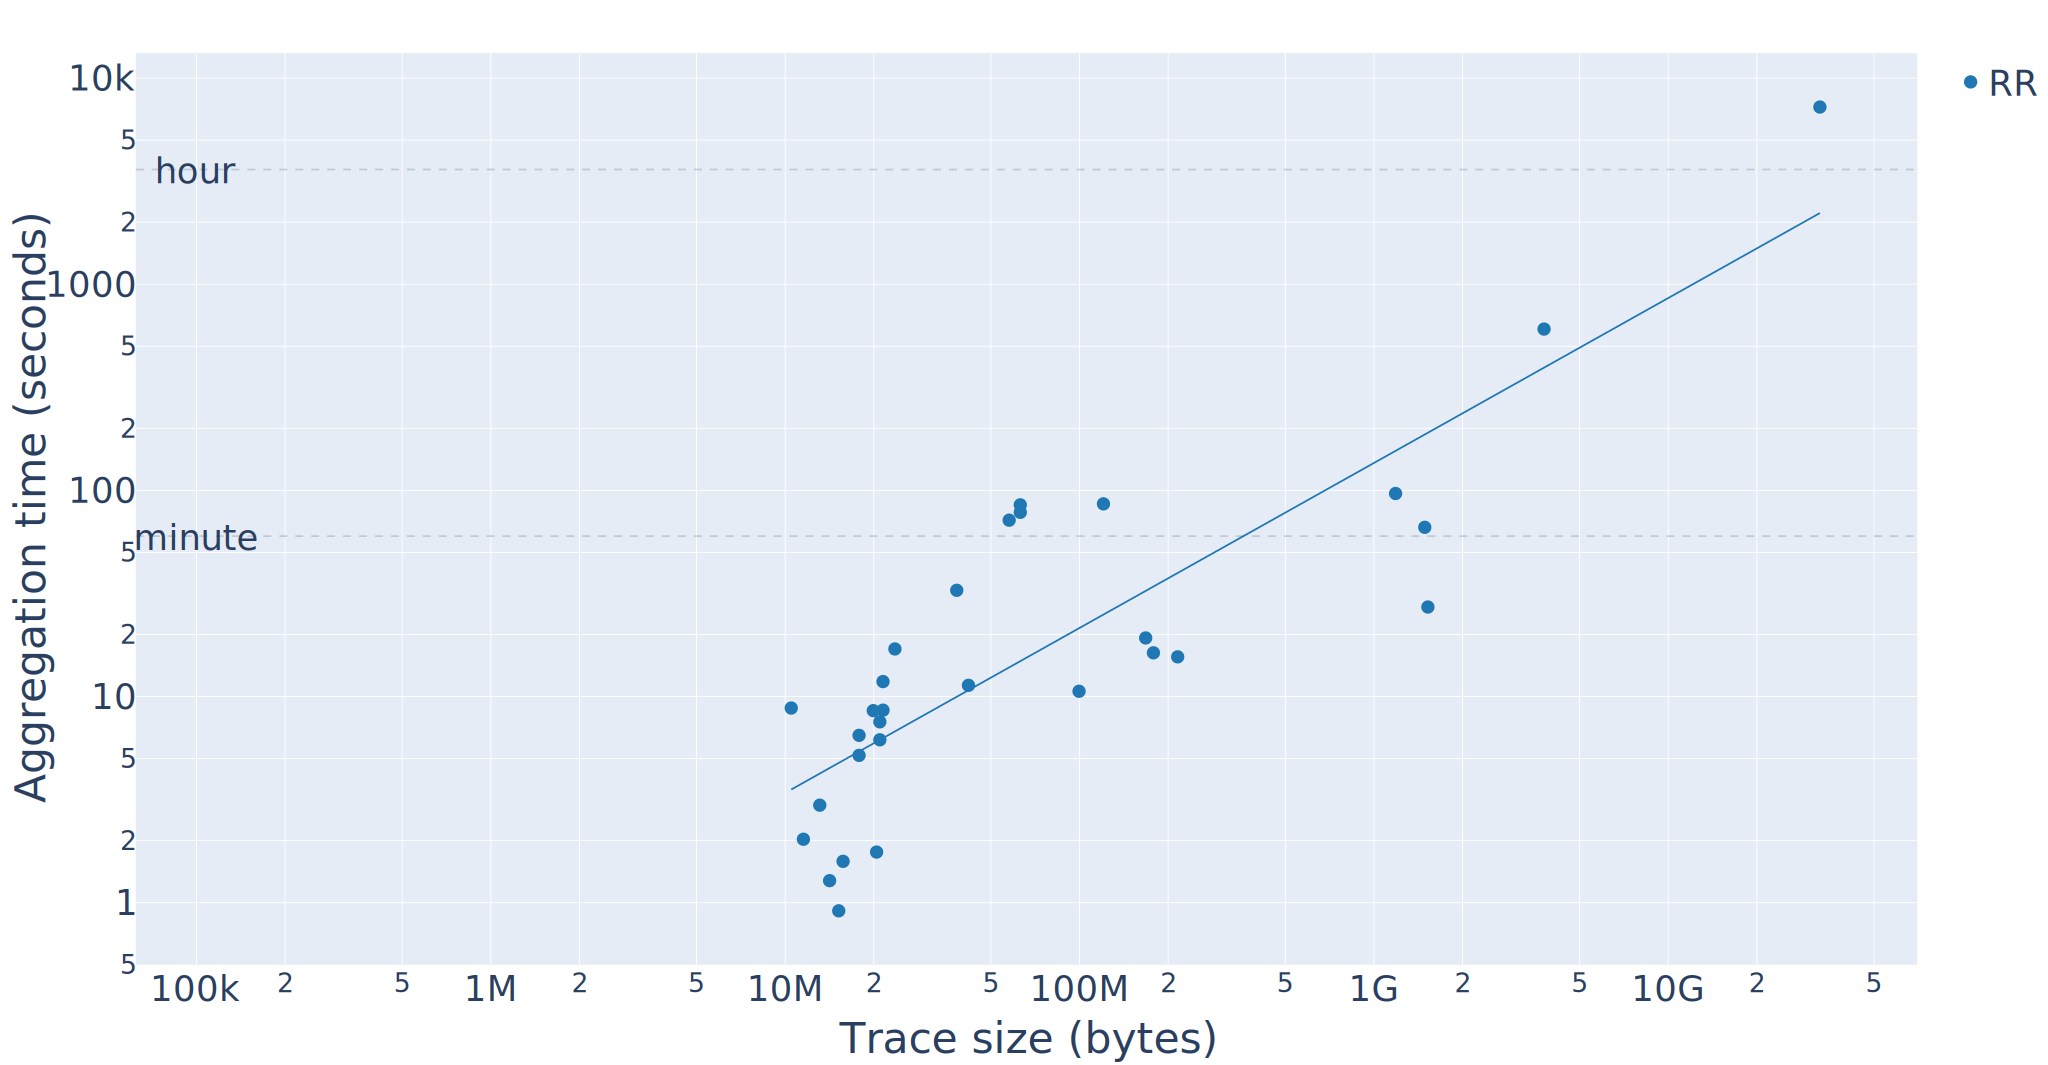
\includegraphics[width=\linewidth]{figure/performance_parsing.pdf}
    \caption{\pytracer aggregation performance. 
    % \tristan{change xlabel to "Trace size (bytes) and ylabel to "Aggregation time (seconds)}
    }
    \label{fig:performance_parsing}
\end{figure}

% \begin{table}
% \centering
% \begin{subfigure}[t]{.75\linewidth}
%     \centering
%     \begin{tabular}{|l|c|c|c|c|}
%     \hline 
%     Application & Original & Pytracer only & RR & MCA \\
%     \hline 
%     Loading & 0.456 & 8.152 & - & - \\
%     \hline
%     discrete\_cosine\_transform & 0.280 & 8.176 & 10.203 & - \\ 
%     fft\_1D & 0.650 & 9.075 & 11.345 & - \\
%     fft\_2D & 0.311 & 9.500 & 11.929  & 16.433   \\
%     \hline
%     interpolation\_1D & 0.377 & 8.803  & 11.954  & -   \\
%     multivariate\_data &0.626 & 8.648 &  12.711  & - \\
%     bspline & 0.109  & 9.050 & 13.396  & 16.830   \\
%     spline\_1D & 0.111 & 8.618 & 10.960   & - \\
%     spline\_2D & 0.655 & 8.649 & 19.424  & - \\
%     \hline
%     broyden\_fletcher\_goldfarb\_shanno &0.475 & 8.292 & 11.033 & 13.685 \\
%     global\_optimization &1.257 & 55.916  & 93.322  & - \\
%     slsqp & 0.469 & 8.192 & 10.795 & 12.439  \\
%     least\_square\_minimization & 0.505 & 10.151  & 13.888 & -  \\
%     nelder\_mead\_simplex & 0.471 & 8.418  & 11.382  & 12.792  \\
%     newton\_conjugate\_gradient & 0.487 & 8.548  & 11.956  & 14.281 \\
%     root\_findings & 0.462 & 8.198  & 10.787   & - \\
%     root\_finding\_large & 0.801 & 11.525 & 41.493   &  82.701  \\
%     root\_finding\_large\_preconditioned & 0.702 & 10.580 & 33.199   & 57.579  \\
%     trust\_region\_exact & 0.482 & 8.170 & 10.400  & 12.524 \\
%     trust\_region\_truncated\_generalized\_lanczos & 0.459 & 8.457 & 11.216 & 13.245  \\
%     trust\_region\_newton\_conjugate\_gradient & 0.479 & 8.538 & 11.179 & 13.488 \\
%     \hline
%     Adaboost &1.388 &14.553 &  20.999 & - \\
%     Bayesian Ridge Regression & 1.086 & 10.344 & 90.299 & -  \\
%     Online classifier comparison & 15.964 & 72.691 & 2104.114 & -  \\
%     K-Means Clustering & 1.621 & 17.614  & 34.005 & 52.902   \\
%     Covariance estimation & 1.357 & 11.755 & 23.964  & -   \\
%     Decision Tree Regression & 1.185 & 11.194 & 15.760 & 15.918  \\
%     Digits Classification & 1.672 & 12.725 & 40.634 & - \\
%     Face Recognition & 32.159  & 74.356 & - & - \\
%     L1 Penalty & 1.568 & 12.591 & 65.547 & 128.220 \\
%     Lasso and elastic net & 1.057 & 9.903 & 17.078 & -  \\
%     Separating hyperplan & 1.376 & 11.532  & 22.333 & 25.036 \\
%     MNIST classification & 19.650 & 37.838 & 402.389  & - \\
%     Multitask Lasso & 1.090 &10.196 & 15.025  & - \\
%     Orthogonal matching & 1.161 & 12.129 & 21.779   & 31.135 \\
%     PCA decomposition & 1.239 & 10.642 & 15.520 & 17.952    \\
%     Robust Linear Regression & 1.370 & 11.144  & 14.280  & - \\
%     Segmentation toy &1.679 & 22.385 & 87.811  & - \\
%     SVM & 1.403 & 11.737 & 23.203 & 24.126   \\
%     Tomography & 11.108 & 40.177  & 1376.134 & -  \\
%     Weighted samples & 1.358 & 11.768 & 21.255 & 20.541   \\
%     \hline
%     \end{tabular}
% \end{subfigure}
%     \caption{\pytracer tracing overhead in seconds. \tristan{what is the unit in this table?}}
%     \label{tab:pytracer_overhead}
% \end{table}

    
% \begin{table}[]
%     \centering
%     \begin{tabular}{c|c|c|c|c}
%          Pytracer & Verificarlo Instrumentation & Backend & Time (hours:minutes:seconds) & Overhead \\
%          \hline 
%          No & No & - & 00:30:51 & 1 \\
%          No & Yes & IEEE & 01:32:56 & 3 \\
%          No & Yes & RR & 16:52:08 & 32 \\
%          Yes & No & - & 03:11:07 & 6  \\
%          Yes & Yes & IEEE & 11:14:33 & 22 \\
%          Yes & Yes & RR & 25:05:54 & 48 \\
%     \end{tabular}
%     \caption{Overheads of \pytracer on PyAFQ experiment with and without fuzzy.}
%     \label{tab:pytracer_overhead}
% \end{table}

% \begin{table}[]
%     \centering
%     \begin{tabular}{c|c|c|c|c}
%          Pytracer & Verificarlo Instrumentation & Backend & Time (hours:minutes:seconds) & Overhead \\
%          \hline 
%          No & No & - & 15 & 1 \\
%          No & Yes & IEEE & 49 & 3 \\
%          No & Yes & RR &  & 441 & 29 \\
%          Yes & No & - & 03:11:07 & 6  \\
%          Yes & Yes & IEEE & 11:14:33 & 22 \\
%          Yes & Yes & RR & 25:05:54 & 48 \\
%     \end{tabular}
%     \caption{Caption}
%     \label{tab:pytracer_overhead}
% \end{table}

Figure~\ref{fig:performance_parsing} shows
the postprocessing time and trace sizes produced by \pytracer. 
The linear correlation between the log of the size and the log of the time shows a significant correlation 
(p-value $\leq 10^{-8}$ for RR and p-value $\leq 10^{-3}$ for MCA).
% \tristan{Mention linear correlation with p-value here.}

In conclusion, while \pytracer's overhead is substantial, it remains tractable for real-life examples.

\section{Discussion}

% Numpy   2509 (2403 not tests) (1848) functions, 1196 (1154) (817) classes (pure Python)
% Scipy   4031 (2187) (506) functions, 1532 (472) (109) classes (pure Python)
% Sklearn 4807 (1010) (81) functions, 546 (417) (41) classes (pure Python)

% \pytracer is a tool for visualizing the numerical quality of function inputs and outputs along the execution of a Python program. It generates numerical traces and post-processes them to measure numerical discrepancies between executions. \pytracer does not require any particular noise model to estimate uncertainties. We tested it with MCA through the fuzzy ecosystem on two broadly used Python libraries.

Through our analysis of SciPy and scikit-learn, we demonstrated \pytracer's scalability, automaticity, and applicability to a wide range of Python program. The relatively low instrumentation overhead of 3.5$\times$ on average enables the analysis of real-scale applications. \pytracer's instrumentation is fully automatic and does not require manual intervention from the user. Furthermore, \pytracer works on any Python libraries, with any data format supported by pickle and any numerical noise model.

\pytracer is the first tool to enable a systematic numerical analysis of Python codes. Existing tools focus on traditional languages of the HPC community, such as C, C++, and FORTRAN. However, Python's high-level abstraction allows for quick application implementations while maintaining high-performance thanks to specialized libraries such as NumPy. Therefore, \pytracer meets the numerical analysis needs of an ever-increasing number of applications.

\pytracer allows users to pinpoint the root causes of numerical instabilities by working at the function level. Numerical stability evaluations are complex since calculations are strongly interdependent. Function-level instrumentation limits the size of the traces since only inputs and outputs of a function are dumped. Moreover, it decreases instrumentation overhead and helps the user identify instabilities quickly. Working at the function level is thus a suitable compromise between analysis conducted at the floating-point operation level and user debug prints. Indeed,  fine-grained analyses are costly and hard to interpret as they overwhelm users with information. In contrast, looking at intermediate results through print statements 
is lightweight but not reliable since developers may not systematically instrument unstable functions. Finally, the SciPy environment wraps many computation kernels written in C, such as BLAS or LAPACK. By working at the function level, \pytracer allows the user to evaluate the numerical precision of such kernels and their impact on the code without getting deep into technical implementation aspects. 

Integrating \pytracer at the early stages of the development cycle would improve the overall numerical quality of the developed code.
\pytracer's automaticity facilitates its usage and enables its integration in unit testing.
For example, \pytracer could be used in regression tests to ensure that updates do not degrade the numerical quality of a calculation. 

\pytracer can also be useful for selecting hyperparameters, as is the case in machine learning.
Indeed, it is common for data scientists to explore a range of hyperparameters and select the ones giving the best scores. With \pytracer, the user has a practical way to quantify numerical quality and understand why hyperparameters produce inconsistent results instead of tweaking hyperparameters to make solvers converge. For instance, the Face Recognition example  (Figure~\ref{fig:face_recognition_svd}) shows how numerical precision could inform the selection of the number of components in dimensionality reduction. 


The visualization provides a global view of the code and interactions between computations. In addition, the Plotly dashboard helps navigate through the code easily, without the need for ad-hoc scripts to visualize data. Finally, the dashboard can be extended to support other data formats to visualize. At this stage, \pytracer currently supports n-dimensional NumPy arrays as well as native Python data. 

As we showed in Section~\ref{sec:impact_mca_modes}, using Full MCA mode leads to runtime errors that have a considerable impact on the proper functioning of the execution, which is unfortunate since these errors do not reflect actual numerical errors but are related to perturbations that should not occur. Conversely, RR mode is far more conservative since it preserves exact operations and is easier to use even though it does not simulate all perturbations. Therefore, from our experiments, we recommend the use of RR over Full MCA. More research is required to address the issues encountered with Full MCA. 

Finally, the wide range of results precision obtained from our experiments demonstrate that looking at the numerical variability is essential and that such analyses would benefit from being conducted systematically.
We showed that well-known scientific libraries are prone to numerical error even though they have been well tested for decades.
The omnipresence of these libraries in scientific codes should thus impel users to integrate numerical analysis in their development workflow in addition to testing their implementation.

\section{Related work}

Several tools have been developed to assess numerical quality, and can be divided into static and dynamic approaches. Static approaches typically analyze source code, while dynamic approaches trace floating-point computations throughout executions. A detailed review of these approaches is presented in~\cite{cherubin2020tools}. 
% \pytracer adopts the dynamic approach due to its scalability to large code bases. Dynamic approaches typically trace floating-point computations, detect instabilities in traces, and visualize summary statistics about instabilities. This section reviews existing approaches for each of these steps. 
% \label{sec:soa}
% \paragraph{Numerical tracing techniques}
Numerous tools exists to trace floating-point computations for C, C++, or FORTRAN programs due to the prevalence of these languages in High-Performance Computing (HPC). 
The main tracing techniques are \textit{source-to-source}, \textit{compiler-based transformations}, and \textit{dynamic binary instrumentation}.

% \gkmod{}{Note: this paragraph just reads like a list with no real interpretation/commentary. I think it would be better to state the strengths of this technique, cite examples, and then state limitations/why it isn't the only technique used.}
The source-to-source technique requires a rewriting of the application to modify floating-point types and provides a fine-grained control on the analyzed code.
CADNA~\cite{jezequel2008cadna} is a library for C, C++, and Fortran implementing  
CESTAC~\cite{vignes1993stochastic} stochastic arithmetic. Shaman~\cite{demeure_phd} is a C++ library that uses a first-order error model to propagate numerical error. 
MCAlib~\cite{frechtling2015mcalib} is a C library that implements the Monte Carlo Arithmetic (MCA)~\cite{parker1997monte} using the MPFR~\cite{fousse2007mpfr} library.
Finally, the work in~\cite{tang2016software} proposed a source-to-source framework for executing targeted code in infinite and fixed precision with and without stochastic arithmetic. The main drawback of the source-to-source approach is its lacks of scalability since rewriting large codes can be a tedious task.
 
% \gkmod{}{Note: similar to the above, this is just a list rather than a highlight of how the compiler-based approach can be more scalable than source-to-source because it requires less manual intervention into a codebase (e.g.), then have your list, and finally say why it is still limited/not a global fix to this problem.}

The compiler-based approach instruments floating-point expressions at compile time
and so allows the user to automatically instrument large codebases.
Verificarlo~\cite{verificarlo} is a compiler that supports different types of arithmetic instrumentations, including MCA. 
The work in~\cite{bao2013fly} modified the GNU Compiler Collection (GCC) to track local floating-point errors across executions. pLiner~\cite{guo2020pliner} is a root-cause analyzer based on the Clang compiler that detects floating-point operations responsible for result variability using a source-to-source transformation at the Abstract Syntax Tree (AST) level to rewrite parts of code with higher precision. 
PFPSanitizer~\cite{chowdhary2020debugging,chowdhary2021parallel} is a compiler that uses parallel shadow execution to detect numerical issues using higher precision.
FLiT~\cite{sawaya2017flit} is a framework to detect variability induced by compilers and their optimizations.
The work in~\cite{wang2012development} proposes a numerical debugger based on GDB~\cite{stallman1988debugging} for Discrete Stochastic Arithmetic (DSA) on FPGA as an Eclipse plugging. Similarly, Cadtrace~\cite{jezequel2008cadna} and Shaman propose a GDB-based tool to use the CADNA and Shaman libraries with GDB, respectively.
The main limitation of the compiler-based approach is that one must have access to the source code.

Dynamic Binary Instrumentation (DBI) operates directly on executables, without the need for recompilation or manual changes. Therefore, it is applicable to any programming language.
CraftHPC~\cite{lam2013dynamic} uses DBI to detect catastrophic cancellations at runtime.
Verrou~\cite{fevotte2016verrou} is a Valgrind~\cite{nethercote2007valgrind} based tool that dynamically replaces
floating-point operations with their stochastic arithmetic counterparts. FPDebug~\cite{benz2012dynamic} uses DBI to detect numerical inaccuracies by using shadow computations with higher precision.
Herbgring~\cite{sanchez2017finding} is a Valgrind-based tool to detect
numerical instabilities. It uses a shadow memory to detect precision losses by comparison with results obtained at higher precision. It is combined with symbolic computation to backtrack the root of the error.
We can note that all methods based on a high-precision oracle suppose that computing with a large number of bits is sufficient to obtain an accurate result, which is not always true (see for example, the famous Muller's sequence~\cite{bajard1996introduction}). 
Although versatile, the DBI looses high-level information useful to understand the source-code logic.

% \gkmod{}{Note: I like this comparison here, but do think that the comments above about providing some more info when each is mentioned would still help this section.}
Being agnostic to the programming language is a serious advantage of the DBI method compared to source-to-source and compiler-bases methods. However, working at the binary level makes it difficult to access high-level information needed to debug and understand the source-code logic. Conversely, the source-to-source approach provides a fine-grained control on the analyzed code, but it lacks scalability, as rewriting large codes can be a tedious task. Finally, the compiler-based approach takes advantage of the best of both by being automatic and having access to high-level information. However, like source-to-source, the compiler-based method is not suitable for analyzing closed-source libraries.

To the best of our knowledge, \pytracer is the first tool dedicated to the numerical analysis of Python code. Existing tools for tracing Python code focus on performance profiling for time (cProfile) 
or memory consumption (memprofile). 
Anteater~\cite{faust2019anteater} is a Python tracer tool to debug Python applications. 
It performs source transformations at the AST level but only deals with native numeric Python types.
Moreover, the user needs to manually tag each variable to trace. Finally, according to the authors, Anteater does not scale to large traces.
cProfile, memprofile, and Anteater use Python decorators as the primary instrumentation technique, a Python mechanism to instrument a function by adding a line over a function declaration.
While this method is appropriate when targeting specific functions, it is not feasible for large codebases where potentially unstable code sections are unknown.


% \label{sec:detecting-instabilities}
% \paragraph{Dynamically detecting numerical instabilities}
% \label{sec:mca}
% :
%  \Yohan{Either detail this section with UA/SA or remove it since MCA is introduced in 'noise injection' subsection. } \tristan{I agree, let's just remove it, the core of the contribution is on the tracing, not in the detection of instabilities.}

% % We review here the existing theoretical framework that might be used to detect numerical instabilities.
% % Our experiments rely on the Monte Carlo Arithmetic (MCA), a stochastic arithmetic allowing 
% % to detect numerical errors by adding random perturbations in the floating-point computations.
% % However, Pytracer do not rely on any assumption about the perturbation model used and thus leaves the user free to use
% % an alternative model. As such, we describe two others options that we thought might be beneficial and complementary to MCA: 
% % input data uncertainty analysis and random seed sensitivity.

% % \subsubsection{Stochastic Arithmetic}

% % The Monte Carlo Arithmetic is a variant of so-called stochastic arithmetic, whose purpose is to model round-off errors by a random variable.

% Three main approaches exist to detect numerical instabilities dynamically: stochastic arithmetic, uncertainty or sensitivity analysis~\cite{helton2006survey}, and random seed analysis~\cite{click2011quality}.
% Stochastic arithmetic leverages randomness to estimate numerical instabilities coming from the use of floating-point representations. The main idea is to treat round-off errors as random variables and characterize them statistically.
% The first published complete stochastic arithmetic framework was CESTAC~\cite{vignes1993stochastic}. In CESTAC, each floating-point computation is performed multiple times with different rounding modes: round-up or round-down. From these stochastic samples, one can then derive the number of significant digits in the computed result. Discrete Stochastic Arithmetic~\cite{vignes2004discrete} extends CESTAC with comparison operators implemented in the CADNA library.
% Monte Carlo Arithmetic (MCA)~\cite{parker1997monte} uses the same principle but introduces two differences:
% (i) a virtual precision parameter, allowing to simulate reduced working precision, and (ii) different perturbation modes to introduce perturbations
% on function inputs or output.
% Stochastic arithmetic quantifies numerical error using the number of significant digits $s$ estimated among the sampled values. A common formula to determine this number from MCA samples is presented in~\cite{parker1997monte}.
% Sohier et al.~\cite{sohier2018confidence} recently provided a generalization of this formula to include confidence intervals.

% % \subsubsection{Uncertainty, sensitivity, and random seed analysis}
% % \tristan{I'm wondering if we could remove this sub-section, as it doesn't seem to be critical to the understanding of the paper, wdyt?}
% % Uncertainty analysis (UA) is a method to estimate the output distribution given an input distribution.
% % Sensitivity analysis (SA) is a variation of UA that measures the local response to a small perturbation~\cite{loucks2017water}. 
% % Several approaches for UA and SA exist, among them differential analysis, response surface methodology, Monte Carlo analysis, and variance decomposition (see~\cite{helton2006survey} for a review). In particular, Monte Carlo analysis is a sampling-based technique that samples inputs space to estimate output response. Monte Carlo analysis shares similarities with Monte Carlo Arithmetic. For instance, the PRECISE framework~\cite{chaitin1996lectures} shares with MCA the idea of varying virtual precision to estimate output sensitivity.

% % Furthermore, the quality of a Random Number Generator is a crucial characteristic when dealing with stochastic model and differ from cryptography requirements. A good RNG provides a tradeoff between performance, period, correlation, or uniformity~\cite{james2020review} for numerical simulation.  
% On the other hand, poor-quality RNGs may have a substantial impact on results~\cite{click2011quality}. First, measuring variation induced by seed is a good indicator of program stability that we can compare against variability induced by floating-point arithmetic.


% \paragraph{Visualization of numerical data}
% \tristan{now that it's here, I'm not sure if this section really adds to the paper. It could also go.}

% Floating-point values approximate real number in the computer arithmetic but
% data manipulated by scientific applications include a large variety of mathematical objects
% beyond scalar values. 
% Indeed, scientific visualization 
% \gkmod{}{Note: You kind of jump right in to this section. Visualization of what in particular? Why do we want (need?) to visualize this sort of data?} 
% covers a wide range of numerical simulation domains, from general-purpose numerical visualization with tools such as VTK~\cite{schroeder2000visualizing} to topological data analysis~\cite{tierny2018topological}, including matrix~\cite{wu2008matrix} or tensor~\cite{kindlmann2006diffusion} visualization.
% To be able to visualize those objects is crucial for the practitioner 
% as information about the structure of the object may be as important as the basic elements that constitute it (i.e. vectors or matrices). 
% Despite the large number of existing tools to identify numerically unstable sections of source code, few allow the user to have a global view of the numerical precision of their computations or to compare several executions of the same program under various perturbations.

% Veritracer~\cite{chatelain2018veritracer} was the first tool to propose an embedded visualizer of numerical stability over the execution of C, C++, and Fortran code. Veritracer extends Verificarlo~\cite{verificarlo} with contextual information about traced variables, which allows the user to identify instabilities quickly.
% However, Veritracer neither offers a dynamic interface nor includes information about high-level structures such as \texttt{struct} or \texttt{array}.
% FPAvizual~\cite{gu2014fpavisual} visualizes the effects of floating-point arithmetic but only for educational purposes and so does not target computational intensive applications\gkmod{}{Q: What does this mean?}.
% Anteater~\cite{faust2019anteater} proposes a visualizer for Python code, but as mentioned previously, it only deals with native Python types, and the user needs to select variables to trace manually. Anteater provides an insightful reflection 
% around visual debugging beyond floating-point analysis, which has inspired the design of \pytracer's visualization interface.

% Through our analysis of SciPy and Scikit-learn, we demonstrated \pytracer's scalability, automaticity, and applicability to any Python program. The relatively low instrumentation overhead of $3.5\times$ on average enables the analysis of real applications. \pytracer's instrumentation is fully automatic and does not require manual intervention from the user. \pytracer works on any Python libraries, with any data format supported by Pickle and any numerical noise model.

% \pytracer is the first tool to enable a systematic numerical analysis of Python codes. Existing tools focus on traditional languages of the HPC community such as C, C++, and FORTRAN. However, Python's high-level abstraction allows for quickly developing applications while maintaining high performance thanks to specialized libraries such as NumPy. Therefore, \pytracer meets the numerical analysis needs of an ever-increasing number of applications.

% Furthermore, \pytracer allows users to pinpoint numerical instabilities root causes precisely by working at the function level. Indeed, evaluating the numerical stability is complex since calculations 
% are strongly correlated between them. 
% The instrumentation at the function level limits the size of the traces since only inputs and outputs of a function are dumped. It moreover decreases the overhead of the instrumentation and helps the user to identify instabilities quickly. 
% Working at function level is thus a suitable compromise between (1) analyzing at the floating-point operation level and (2) user debug prints.
% (1) Indeed, the fine-grained analysis is costly and hard to analyze due to the large amount of computations evolved in HPC codes. It overwhelms the user with too much information, making analysis more difficult but can be interesting at the final step of the understanding. 
% (2) Looking at intermediate results through print statements focuses on valuable information
% (like residuals or norms) but may miss numerically unstable functions unsuspected by the developer.
% Finally, the SciPy environment wraps a lot of computation kernels written in C, like BLAS or LAPACK.
% By working at function level, \pytracer allows the user to evaluate the numerical precision of such kernels
% and their impact on the code without getting deep into technical implementation aspects. 

% Python is a popular language to prototype proof-of-concept. Integrating \pytracer at early stages of the development cycle allows identifying numerical instabilities to write code of better quality.
% \pytracer's automaticity facilitates the usage and enables its integration in unit testing.
% It can be for example used in a non-regression test to ensure that the numerical quality of a calculation
% is not degraded by updates. Moreover, the Plotly dashboard offers a quick visualization to 
% analyze more finely the potential issues.

% \pytracer can also be useful to select the hyperparameters of a code, as it is the case in machine learning.
% Indeed, we find many cases in the literature where users explore a range of hyperparameters
% to select the ones giving the best scores. With \pytracer, 
% the user has a practical way to quantify the numerical quality and to understand why hyperparameters
% lead to unstable outputs, instead of tweaking hyperparameters to make solvers converge, 

% The visualization permits a global view of the code and to understand interactions between 
% computations. The Plotly dashboard help to easily navigate through the code.
% It moreover removes the need for ad-hoc scripts to visualize data. 
% Finally, the dashboard can be extended to support other data format to visualize.
% \pytracer currently supports n-dimensional NumPy arrays as well as native Python data. 

% As we showed in Section~\ref{sec:impact_mca_modes}, using Full MCA mode leads to runtime errors that have a considerable impact on the proper functioning of the execution. This is unfortunate since these errors do not reflect actual numerical errors but errors related to perturbations that should not occur.
% Conversely, RR mode is far more conservative since it preserves exact operations and is easier to use even though it does not simulate all perturbations.
% From our experiments, we do not recommend the Full MCA mode for now and more researches are needed 
% to help fixing issues we encountered.

% Fixing this issue would enable the study of catastrophic cancellations, which are common sources of numerical errors. 
% In addition to the runtime errors it raises, mismatching shapes is also a problem when aggregating traces as \pytracer will not compute statistics for a set of arrays with different shapes \tristan{So do you conclude that Full MCA is not usable while RR is? If so, you should recommend to use Pytracer with RR only.} \tristan{are you still talking about Full MCA here? if not, make another paragraph. If so, make it clearer.}. Two solutions exist to overcome this issue: the first is not to instrument the \texttt{PyArray\_Arange} function with MCA. The advantage is that it is easy to set up since it requires one extra line in the exclusion file. However, the same kind of problem may appear somewhere else because, as we have seen, the evolved operations are elementary. Therefore, the chances that developers reproduce the same pattern are very probable. Therefore, the second solution is to ensure that the Full MCA mode preserves the exact operations. This solution has the advantage of not worrying about which functions should be instrumented or not with MCA, but it is hard to achieve it in practice. Indeed, we rely on the MCA implementation provided by Verificarlo that uses an internal precision to add the random perturbation that is higher than the working precision for applying the random noise. Verificarlo then rounds the result to the working precision before returning it, so any residual noise lower than the working precision is lost. Keeping track of that noise would require recording each intermediate computation in a shadow memory or keeping a tag about their exactness. This option would require more extra works than the first one but would ensure more consistent results. \tristan{I find this paragraph too verbose, you should contract it to a few key sentences.}

% \tristan{The following paragraphs are future work, not discussion. I'd remove them and flesh out the discussion from the ideas mentioned in the current 3rd paragraph}

% Also, we would like to extend the post-process analysis to aggregate traces where the execution flow path diverges. Therefore, a posteriori reconstruction is challenging as one must precisely identify the flow path taken and find synchronization points to pursue the analysis. We retrieve, for example, this divergence behavior in two general classes of numerical schemes: iterative methods and optimization processes. One solution is to integrate methods used in code coverage analysis to keep track of flow paths taken and the backtraces. However, this would increase the complexity of the postprocess analysis as well as an extra slowdown factor. However, by coupling the Gantt chart with static analysis, \pytracer would catch some divergence patterns occurring within a function. Indeed, by instrumenting at the function level, \pytracer views the function's callees (i.e., the functions called within a function) and thus should partially detect flow divergences.

% By design principle, \pytracer is flexible on the noise model used, although we only tested it with the MCA model in our experiments. Nevertheless, we would like to compare different models against MCA in future works to see the resulting differences. Furthermore, we would like to test \pytracer on parallel codes.

% Finally, we would extend \pytracer to instrument elementary arithmetic operations which can be helpful to more profound analyses. We nevertheless believe that instrumentation at the function level presents two advantages: it first limits the size of the traces since only inputs and outputs of a function are saved instead of a full report which, on the one hand, decreases the overhead of the instrumentation and, on the other hand, help the user to identify instabilities quickly. Indeed, full reporting can overwhelm the user with too much information, making analysis more difficult at first. Second, the analysis at fine granularity is interesting at the final step of the understanding. Such an analysis would require a different instrumentation approach by, for example, working at the Abstract Syntax Tree (AST) level since it is trivial to get it in Python.
% Moreover, working at the AST level allows doing dependency analysis. Another extension would be to extract and replay a function, in the same vein as the CERE tool does but for Python, and to use an AST instrumentation to analyze the numerical quality of elementary operations step by step within the fuzzy environment.



% \pytracer is a tool for visualizing the numerical quality of function inputs/outputs over time.
% It generates numerical traces that are aggregated in postprocessing to measure numerical discrepancies between executions.
% \pytracer does not assume the noise model used to estimate uncertainties but has been tested with the MCA 
% through the fuzzy ecosystem on two broadly used scientific libraries for Python with partial success.

% We demonstrated the Pytracer's capabilities to analyze intensively used Python libraries such as NumPy or Scikit-learn, such as 
% 1) Scalability. The low instrumentation overhead of 3.5x enables analysis of real applications and permits having a global representation of the numerical quality of an application. 
% 2) Automaticity. Pytracer instrumentation is fully automatic and does not require manual intervention from the user, allowing the instrumentation of 
% the NumPy, SciPy and Scikit-learn libraries.
% // that cumulate 5600 and 2043 pure Python functions and classes. 
% 3) Agnosticity. Pytracer works on any python libraries, with any data format supported by pickle, and any numerical noise model flavor.

% Pytracer is the first tool to bring numerical analysis of Python codes available to everyone. Indeed, existing tools developed in the last years focused on traditional HPC languages community such as C,C++, and FORTRAN. However, the Python high-level abstraction allows you to quickly develop applications while maintaining high performance with the help of specialized libraries like NumPy. Therefore, it is quite natural to see more fields systematically using Python, as is the case in neuroimaging. Thus, Pytracer meets the numerical analysis needs of an ever increasing number of applications writing in Python.

% By working at function level, Pytracer allows users to precisely pinpoint numerical instabilities root causes. Furthermore, the automaticity facilitates the usage and its integration in unit testing. Hence, instead of tweaking hyperparameters to make solvers converging, the user has a practical way with Pytracer to quantify the numerical quality of its computations. 

% As we showed in section~\ref{sec:impact_mca_modes}, using the Full MCA mode leads to runtime errors that have a considerable impact on the proper functioning of the execution, which is unfortunate since these
% errors do not reflect actual numerical errors but errors related to perturbations that should not occur.
% Fixing this misbehavior would greatly help use Full MCA mode since this mode allows simulating catastrophic cancellations, which are familiar sources of numerical errors. By preserving exact operations, RR mode is far more conservative and so easy to use even though it does not simulate all perturbations that might be encountered. 

% Also, using a post-process analysis to aggregate traces, \pytracer falls in the same pitfalls as veritracer and is limited to aggregate traces where the execution flow path extremely diverges. Therefore, a posteriori reconstruction
% is challenging as one must precisely identify the flow path taken and find synchronization points to pursue the analysis. We retrieve, for example, this divergence behavior in two general classes of numerical schemes: iterative methods and optimization processes. One solution to overcome this issue is to integrate methods used in code coverage analysis to keep track of flow paths taken and the backtraces.
% However, this would increase the complexity of the postprocess analysis as well as an extra slowdown factor.
% However, by coupling the Gantt chart with static analysis, \pytracer would catch some divergence patterns occurring within a function. Indeed, by instrumenting at the function level, \pytracer views the function's callees (i.e., the functions called within a function) and thus should partially detect flow divergences.

% By design principle, \pytracer is flexible on the noise model used, although we only tested it with the MCA model in our experiments.
% Nevertheless, we would like to compare different models against MCA in future works to see the resulting differences. 
% In particular, although \pytracer only works on a sequential application for the moment, it can be used to analyze parallel sections internal to a function.
% The only restriction is that the section does not call other functions traced by \pytracer; we would fall into the previous issue of divergence if it would not be the case.
% Since \pytracer only cares about inputs and outputs of a function, the order of internal operations is transparent for it and thus should be able to handle those cases.

% Finally, \pytracer does not instrument elementary arithmetic operations, and it can be a barrier to more profound analysis.
%Such an analysis would require a different instrumentation approach by, for example, working at the Abstract Syntax Tree (AST) level since it is trivial to get it in Python.
% An ideal way to do that would be to extract and replay a function, in the same vein as the CERE~\cite{castro2015cere} tool does but for Python, and use an AST instrumentation to analyze the numerical quality of elementary operations step by step within the fuzzy environment.
% Lastly, AST analysis can serve as a basis for finding relationships between variables, valuable information for the user.

% In addition to the runtime errors it raises, mismatching shapes is also a problem when aggregating traces as PyTracer will not compute statistics for a set of arrays with different shapes.
% Two solutions exist to overcome this issue: the first is not to instrument the \texttt{PyArray\_Arange} function with MCA. The advantage is that it is easy to set up since it requires one extra line in the exclusion file.
% However, the same kind of problem may appear somewhere else
% because, as we have seen, the operations being evolved are elementary. Therefore, the chances that developers reproduce the same pattern are very probable. The second solution is to ensure that the Full MCA mode preserves the exact operations.
% This solution has the advantage of not worrying about which functions should be instrumented or not with MCA, but it is hard to achieve it in practice. Indeed, we rely on the MCA implementation provided by Verificarlo that uses an internal precision to add the random perturbation that is higher than the working precision for applying the random noise. Verificarlo then rounds the result to the working precision before returning it, so any residual noise lower than the working precision is lost. 
% Keeping track of that noise would require recording each intermediate computation in a shadow memory or keeping a tag about their exactness.
% \Yohan{This idea emerged by discussing with Verificarlo's team. 
% I must find a way to express that and not give the impression that we discovered or suggest it.}
% This option would require more extra works than the first one but would ensure more consistent results.

\section{Conclusion}


% \tristan{I moved this from the opening of Section 4, as this reads more like a summary of \pytracer's features than an experiment description. It should be refactored in 1-2 paragraphs summarizing the main properties of \\pytracer.}

Evaluating the numerical stability of scientific Python programs is a tedious task that requires substantial expertise. Automatic tools to help users understand the behavior of their code are therefore crucial.
In this perspective, \pytracer is the first tool to offer a complete framework for analyzing and visualizing the numerical stability of Python codes. It works by automatically instrumenting Python libraries to produce numerical traces visualized through an interactive Plotly Dash server. \pytracer does not require manual code modification, and we tested it with major scientific libraries such as NumPy, SciPy, and Scikit-learn. Our results show that \pytracer is scalable, with an average instrumentation slowdown of $3.5\times$. Moreover, \pytracer's visualization interface remains responsive even with traces of up to 1TB. 
In our experiments, \pytracer enabled the systematic evaluation of 40 examples from the SciPy and scikit-learn libraries. 

In future work, we plan to extend the post-processing analysis to aggregate traces when the execution flow path diverges by leveraging techniques used in code coverage analysis. Moreover, we would like to extend \pytracer to instrument elementary arithmetic operations which can be helpful to more profound analyses. Finally, although \pytracer supports multiple noise models, we only tested it with Monte Carlo Arithmetic. Therefore, we would like to compare different models against MCA. 
\pytracer is available at \href{https://github.com/big-data-lab-team/pytracer}{github://big-data-lab-team/pytracer} under MIT License.

% Evaluating the numerical stability of scientific Python codes is a tedious task
% and requires an expertise to be conducted. Automatic tools to help the users 
% understanding what's going on in their codes is therefore crucial.
% In this perspective, \pytracer is the first tool to offer a complete framework
% for analyzing and visualizing the numerical stability of Python codes.
% It works by automatically instrumenting Python libraries to produce numerical
% traces visualized through an interactive Plotly Dash server.
% \pytracer does not require manual code modification, and has been tested with 
% major scientific libraries such as NumPy, SciPy, and Scikit-learn. Our results show that \pytracer is scalable, with an average instrumentation slowdown of $3.5\times$. \pytracer's visualization interface remains responsive even with traces of up to 1TB. Moreover,
% \pytracer is by construction agnostic to the noise model used 
% to evaluate the numerical stability. We have demonstrated 
% that \pytracer can be used with the Monte Carlo Arithmetic 
% through the fuzzy environment. 
% The experiments conducted in this paper are the first largest application of the fuzzy ecosystem by the wide range of applications covered. 

% In future work, we would like to extend the post-process analysis to aggregate traces 
% when the execution flow path diverges by leveraging techniques used in code coverage analysis.
% Moreover, we would like to extend \pytracer to instrument elementary arithmetic operations 
% which can be helpful to more profound analyses. Finally, although \pytracer is flexible on the noise
% model used, we only tested it with the Monte Carlo Arithmetic. We would like to compare different 
% models against MCA. 


% We also have to provide feedback about pitfalls and benefits encountered to shed light on first-time users' good and bad practices and democratize MCA's usage. 


% \begin{itemize}

%     \item Domain agnostic: \pytracer is intended to work on any scientific Python applications, without specific domain-specific languages or needs to rely on specific libraries.
%     We target two of the most common libraries used in scientific computing within Python, SciPy and Scikit-learn, and a domain-specific application in neuroimaging. We show that \pytracer works well on these libraries, capturing most of the functions' module targeted.

%     \item Automatic: \pytracer objective is to offer automatic instrumentation for Python applications,
%     from small prototypes to state-of-the-art scientific libraries. 

%     \item Scalable: \pytracer goal is to trace real-world application and use case.
%     In that perspective, we use \pytracer on PyAFQ, a domain-specific neuroimaging application to compute tractograms, generating \pytracer traces up to 1TB. We demonstrate that \pytracer can handle this volume of data and offer the user an interactive and fluent visualization.
%     We also show that \pytracer instrumentation gives a slowdown of $\times 6$.

%     \item Fuzzy compatible: \pytracer aims at evaluating numerical stability by using an injection noise model.
%     Although the noise model used is orthogonal to \pytracer tracing mechanism, we emphasize in these experiments the MCA model through the fuzzy environment and discuss its compatibility with \pytracer tracing mechanism to point out limitations of the trace-based approach and to propose research tracks to overcome them.
%     The experiments conducted in this paper are the first largest application of the fuzzy ecosystem by the wide range of applications covered. We, therefore, found it interesting to give feedback about pitfalls and benefits encountered
%     in order to shed light on the good and bad practices for first-time users and democratize MCA's usage.
%     Moreover, these analyses will help the fuzzy developers to increase the overall stability of fuzzy.

% \end{itemize}

\bibliographystyle{abbrv}
\bibliography{paper}

%%
%% If your work has an appendix, this is the place to put it.
\appendix

\end{document}
\endinput
%%
%% End of file `sample-authordraft.tex'.
